\documentclass[aspectratio=169]{beamer}

\usepackage{amsmath, amssymb, amsxtra, amsthm, amsfonts}
\usetheme{moloch}
\usecolortheme{beaver}
\setbeamertemplate{footline}
{
  \leavevmode%
  \hbox{%
    \begin{beamercolorbox}[wd=.5\paperwidth,ht=2.25ex,dp=1ex,center]{author in head/foot}%
      \usebeamerfont{author in head/foot}\insertsection
    \end{beamercolorbox}%
    \begin{beamercolorbox}[wd=.5\paperwidth,ht=2.25ex,dp=1ex,right]{date in head/foot}%
      \usebeamerfont{date in head/foot}\inserttitle\hspace*{2em}
      \insertframenumber{} / \inserttotalframenumber\hspace*{2ex}
    \end{beamercolorbox}}%
  \vskip0pt%
}
\makeatother

\usepackage[english]{babel}
\usefonttheme{serif}

\usepackage{mathtools}
\usepackage{graphicx}
\usepackage{bm}
\usepackage{color}
\usepackage[dvipsnames,table]{xcolor}
\usepackage{tikz}
\usepackage{stanli}
\usepackage{verbatim}
\usepackage{tikz}
\usetikzlibrary{shapes,calc,through,3d,patterns}
\usetikzlibrary{decorations.pathreplacing}
\usetikzlibrary{arrows.meta,calc,positioning}

\usepackage{pgfplots}
\usepackage{siunitx} % For formatting numbers
\usepackage{hyperref}
\hypersetup{colorlinks=true,linkcolor=darkred}
\usepackage{multicol}
\usepackage[absolute,overlay,]{textpos}
\usepackage{pgfplots}
\pgfplotsset{width=10cm,compat=1.9}
\usepackage{subcaption}
\usepackage{multirow}
\usepackage{bbding}
\usepackage{arydshln}
\usepackage{mathtools}
\usepackage{tcolorbox}
\usepackage{animate}

\textblockorigin{80mm}{45mm}


\newtheorem{thm}{Theorem}
\newtheorem{cor}[thm]{Corollary}
\newtheorem{prop}[thm]{Proposition}
\newtheorem{lem}[thm]{Lemma}
\theoremstyle{remark}
\newtheorem*{rem}{Remark}

%Block def
\definecolor{darkred}{rgb}{0.6,0,0}
\setbeamertemplate{blocks}[rounded][shadow=false]
\setbeamercolor{block title}{bg=darkred!15,fg=black}
\setbeamercolor{block body}{bg=darkred!5,fg=black}

\setbeamercolor{itemize item}{fg=darkred}
\setbeamercolor{itemize subitem}{fg=darkred}
\setbeamercolor{itemize subsubitem}{fg=darkred}
\setbeamercolor{enumerate item}{fg=darkred}
\setbeamercolor{button}{bg=gray!30,fg=darkred}

\setbeamertemplate{itemize item}[square]
\setbeamertemplate{itemize subitem}[circle]
\setbeamertemplate{itemize subsubitem}[triangle]
\setbeamertemplate{enumerate items}[circle]
\setbeamercolor{item projected}{bg=darkred}

\newcommand{\bolddelta}{\boldsymbol\delta}
\newcommand{\boldxi}{\boldsymbol\xi}
\DeclareMathOperator*{\A}{\text{\raisebox{-0.2cm}{\Huge A}}}




\title{Dynamic finite element analysis of structures}
\subtitle{A mathematical perspective}
\author{Stefano Burzio}
\institute{@ Flexlab}
\date{27.01.2026}

\begin{document}
\usenavigationsymbolstemplate{}
{\setbeamertemplate{footline}{}

\frame{\titlepage
  \begin{tikzpicture}[overlay, remember picture]
    \node[anchor=north east, xshift=-.9cm] at (current page.north east) {
\includegraphics[width=2cm]{../images/epfl_logo.png}};
    \node[anchor=south east, xshift=-.87cm, yshift=.05cm] at (current page.south east)  {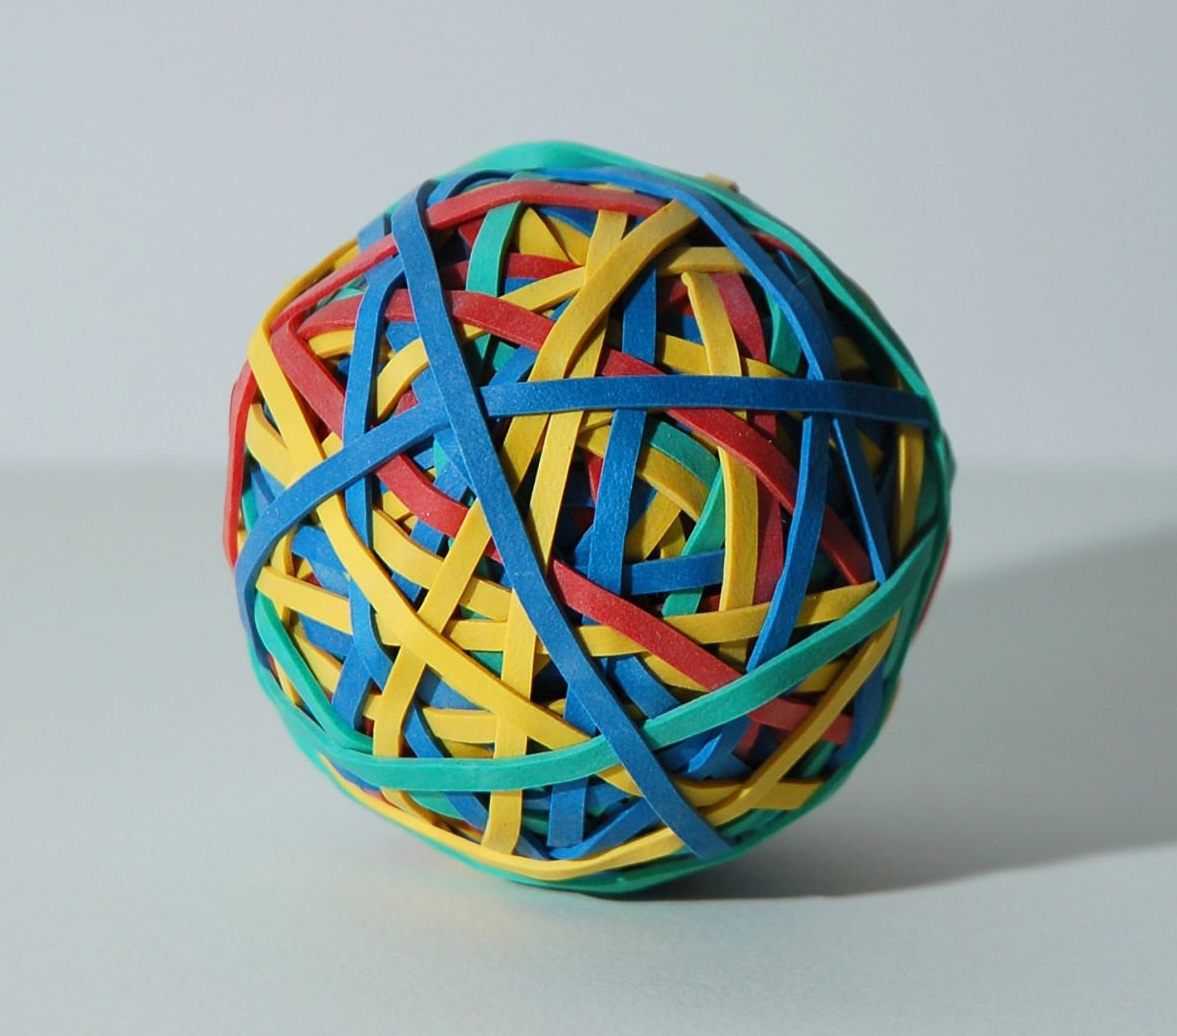
\includegraphics[width=5cm]{../images/rubber_band_ball.jpg}};
  \end{tikzpicture}
}

\section{Strong and weak form of elastodynamics}


 {%backgorund 
  \setbeamertemplate{background canvas}{
\begin{tikzpicture}
      \useasboundingbox (0,0) rectangle (\paperwidth,\paperheight);
      \fill [color=darkred!80] (0.5\paperwidth,0) rectangle (\paperwidth,\paperheight);
    \end{tikzpicture}}



  \begin{frame}
    \begin{columns}
      % Left column with images
      \column{0.55\textwidth}
      \vspace{0.5cm}

      \hspace{0.1cm} 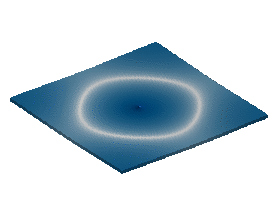
\includegraphics[width=2.5cm]{../images/modePlate1} \hspace{1cm} 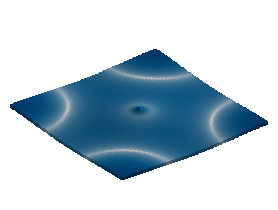
\includegraphics[width=2.5cm]{../images/modePlate2}

      \hspace{0.1cm} 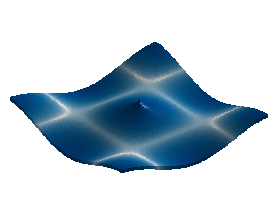
\includegraphics[width=2.5cm]{../images/modePlate3}  \hspace{1cm} 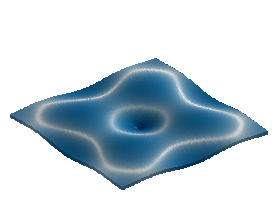
\includegraphics[width=2.5cm]{../images/modePlate4}

      \hspace{0.1cm} 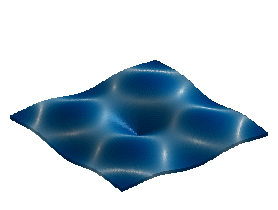
\includegraphics[width=2.5cm]{../images/modePlate5}  \hspace{1cm} 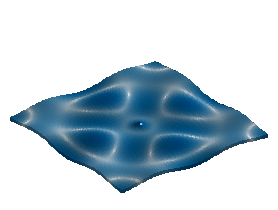
\includegraphics[width=2.5cm]{../images/modePlate6}

      \hspace{0.1cm} 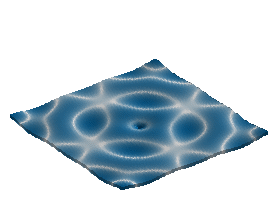
\includegraphics[width=2.5cm]{../images/modePlate7}  \hspace{1cm} 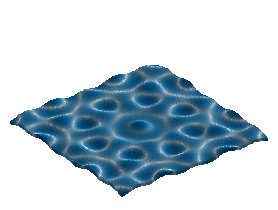
\includegraphics[width=2.5cm]{../images/modePlate8}

      \hspace{0.2cm}\tiny (Credit: \href{https://nojigon.webs.upv.es/simulations_plate.php}{\textcolor{darkred}{Noé Jiménez})}

      % Right column with red background and text
      \column{0.45\textwidth}
      \parbox{\linewidth}{%
        \textbf{\textcolor{white}{\large Linear:}} \textcolor{white}{infinitesimally small deformations relative to the solid's size.} \\[0.9cm]
        \textbf{\textcolor{white}{\large Elasticity:}} \textcolor{white}{deformable material that returns to its original shape and size when the forces causing the deformation are removed.} \\[0.9cm]
        \textbf{\textcolor{white}{\large Dynamics:}} \textcolor{white}{study bodies in motion under the influence of time-dependent loads applied to them.}
      }
    \end{columns}
  \end{frame}
 }

\begin{frame}{Hypothesis and notations}
  \begin{columns}[T]
    \begin{column}{.69\textwidth}
      \begin{itemize}
        \item Inertial orthonormal reference frame $O(x,y,z)$. \\ Sometimes will use $O(x_{1},x_{2},x_{3})$.
        \item Continuous three-dimensional deformable finite (compact) \textbf{body} $\Omega$ with surface $\Gamma$.
        \item \textbf{Material}: continuous and homogenous.
        \item \textbf{Material properties}: $\mathbf C$ and $\rho$.
        \item \textbf{Deformations}: small (proportional to stress).
              \begin{center}
                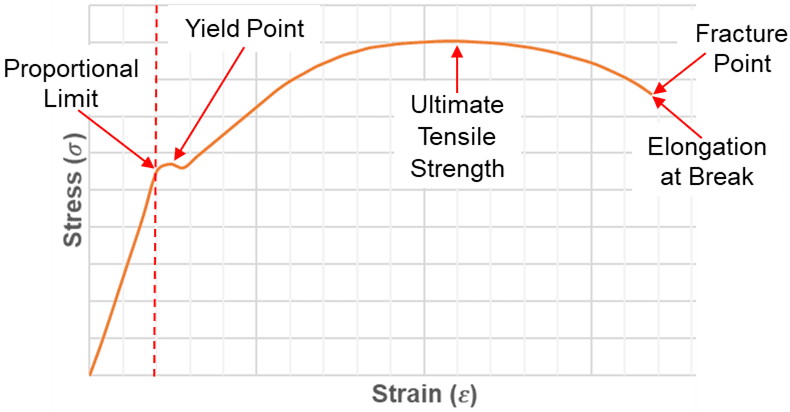
\includegraphics[width=5cm]{../images/strssStrainRelationship.png}
                \newline\noindent{\tiny\emph{Credit: \href{https://www.fidelisfea.com/post/stress-and-strain-what-are-they-and-what-is-their-relationship}{\textcolor{darkred}{Fidelis}}}}
              \end{center}
      \end{itemize}
    \end{column}\hspace{-1.5cm}
    \begin{column}{.4\textwidth}
      \vspace{1cm}
      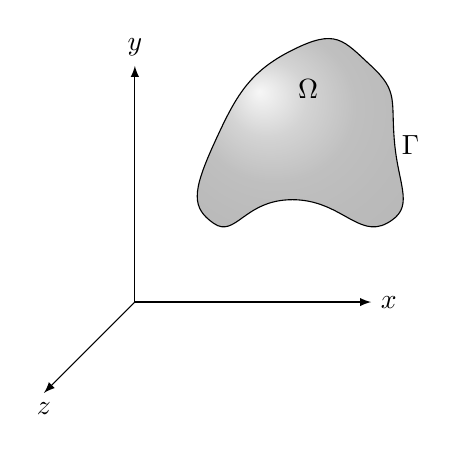
\begin{tikzpicture}
        \draw[-latex] (0,0,0) -- (3,0,0) node[right]{$x$};
        \draw[-latex] (0,0,0) -- (0,3,0) node[above]{$y$};
        \draw[-latex] (0,0,0) -- (0,0,3) node[below]{$z$};
        % Draw the potato-like shape
        \shade [ball color= gray!50!black, opacity=.3] plot [thick,smooth cycle, tension=1] coordinates  {(1,2) (2,3.2) (3,3) (3.3,2) (3.2,1) (2,1.3) (1,1)};
        \draw plot [thick,smooth cycle, tension=1] coordinates {(1,2) (2,3.2) (3,3) (3.3,2) (3.2,1) (2,1.3) (1,1)};
        % Label the region Omega	
        \node at (2.2,2.7) {$\Omega$};
        % Label the boundary Gamma
        \node at (3.5,2) {$\Gamma$};
      \end{tikzpicture}
    \end{column}
  \end{columns}
\end{frame}

\begin{frame}{Undeformed and deformed solid}
  \begin{itemize}
    \item \textbf{Unknown:} displacement $\mathbf u\in C^{2}(\bar\Omega\times[0,T],\mathbb R^{3})$
  \end{itemize}
  \vspace{-0.3cm}
  \begin{columns}[T]
    \begin{column}{.5\textwidth}
      \begin{center}
        \textbf{Undeformed solid}
        \vspace{0.5cm}
        \newline
        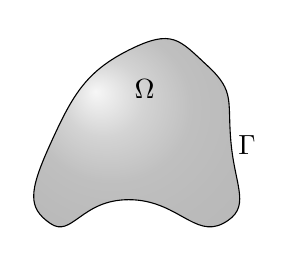
\begin{tikzpicture}
          % Draw the potato-like shape
          \shade [ball color= gray!50!black, opacity=.3] plot [thick,smooth cycle, tension=1] coordinates  {(1,2) (2,3.2) (3,3) (3.3,2) (3.2,1) (2,1.3) (1,1)};
          \draw plot [thick,smooth cycle, tension=1] coordinates {(1,2) (2,3.2) (3,3) (3.3,2) (3.2,1) (2,1.3) (1,1)};
          % Label the region Omega	
          \node at (2.2,2.7) {$\Omega$};
          % Label the boundary Gamma
          \node at (3.5,2) {$\Gamma$};
        \end{tikzpicture}
      \end{center}
    \end{column}
    \hfill
    \begin{column}{.5\textwidth}
      \begin{center}
        \textbf{Deformed solid}
        \vspace{0.5cm}
        \newline
        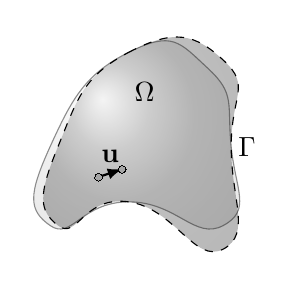
\begin{tikzpicture}
          % Draw the potato-like shape
          \shade [ball color= gray!90, opacity=.1] plot [thick,smooth cycle, tension=1] coordinates  {(1,2) (2,3.2) (3,3) (3.3,2) (3.2,1) (2,1.3) (1,1)};
          \draw[color=gray!90] plot [opacity=.1,smooth cycle, tension=1] coordinates {(1,2) (2,3.2) (3,3) (3.3,2) (3.2,1) (2,1.3) (1,1)};
          \shade [ball color= gray!50!black, opacity=.3] plot [thick,smooth cycle, tension=1] coordinates  {(1.1,2) (2,3.2) (3.2,3.1) (3.3,2) (3.2,0.7) (2,1.3) (1.1,1)};
          \draw[dashed] plot [color=gray!40!black, opacity=.3,thick, smooth cycle, tension=1] coordinates {(1.1,2) (2,3.2) (3.2,3.1) (3.3,2) (3.2,0.7) (2,1.3) (1.1,1)};
          % Label the region Omega	
          \node at (2.2,2.7) {$\Omega$};
          % Label the boundary Gamma
          \node at (3.5,2) {$\Gamma$};
          \draw[thick,-latex] (2,2,1) to node[midway,above]{$\mathbf u$} (2.3,2.1,1);
          \node[draw,shape=circle,fill=black!35,minimum size=1mm,line width=0mm,inner sep=0] at (2,2,1) {};
          \node[draw,shape=circle,fill=black!35,minimum size=1mm,line width=0mm,inner sep=0] at (2.3,2.1,1) {};
        \end{tikzpicture}
      \end{center}
    \end{column}
  \end{columns}
\end{frame}

\begin{frame}{Loads, boundary conditions and initial conditions}
  \begin{columns}[T]
    \begin{column}{.62\textwidth}
      \begin{itemize}
        \item \textbf{Boundary:} $$\Gamma=\Gamma_{u}\cup\Gamma_{\sigma}$$

        \item \textbf{Loads:}
              \begin{itemize}
                \item Acting loads on the body: $\mathbf f$.
                      \vspace{0.1cm}
                \item Boundary conditions:
                      \begin{itemize}
                        \item prescribed displacements $\mathbf{\hat u}$ on the boundary $\Gamma_{u}$,
                        \item prescribed loads $\mathbf{\hat f}$ on the boundary on $\Gamma_{\sigma}$.
                      \end{itemize}\end{itemize}
              \vspace{0.1cm}
        \item \textbf{Initial conditions:} at $t=0$
              \begin{itemize}
                \item initial displacement $\mathbf u_0$
                \item initial velocity $\mathbf v_0$.
              \end{itemize}
      \end{itemize}
    \end{column}
    \hfill
    \begin{column}{.4\textwidth}
      \begin{center}
        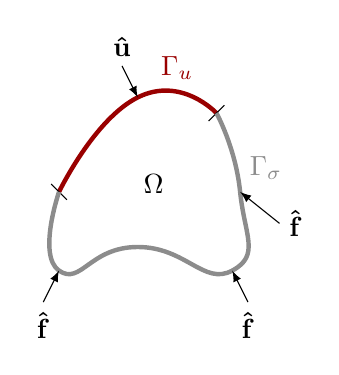
\begin{tikzpicture}
          % Label the region Omega	
          \node at (2.2,2.1) {$\Omega$};
          % Label the boundary Gamma
          \draw[ultra thick, darkred] plot [smooth, tension=1] coordinates {(1,2) (2,3.2) (3,3)};
          \node[darkred, above] at (2.5,3.3) {$\Gamma_u$};
          \draw[thin] (3+0.1,3+0.1) --(3-0.1,3-0.1);
          \draw[thin] (1+0.1,2-0.1) --(1-0.1,2+0.1);
          \draw[latex-]  (2,3.2) --  (2-0.2,3.2+0.4) node[above] {$\mathbf{\hat u}$};
          % Draw part of the boundary Gamma_sigma
          \draw[ultra thick, gray!90] plot [smooth, tension=1] coordinates {(3,3) (3.3,2) (3.2,1) (2,1.3) (1,1) (1,2)};
          \node[gray!90, right] at (3.3,2.3) {$\Gamma_\sigma$};
          \draw[latex-]  (1,1) --  (1-0.2,1-0.4) node[below] {$\mathbf{\hat f}$};;
          \draw[latex-]  (3.2,1) --  (3.2+0.2,1-0.4) node[below] {$\mathbf{\hat f}$};
          \draw[latex-]  (3.3,2) --  (3.3+0.5,2-0.4) node[right] {$\mathbf{\hat f}$};
        \end{tikzpicture}
      \end{center}
    \end{column}
  \end{columns}
\end{frame}


\begin{frame}{Stress and strain tensors}
  \begin{columns}[T]
    \begin{column}{.33\textwidth}
      \small\centering \textbf{Stress tensor}
      $$\boldsymbol{\sigma}(\mathbf x,t)=\begin{bmatrix}\sigma_{11}(\mathbf x,t)\\ \sigma_{22}(\mathbf x,t)\\ \sigma_{33}(\mathbf x,t)\\ \sigma_{23}(\mathbf x,t)\\ \sigma_{31}(\mathbf x,t)\\ \sigma_{12}(\mathbf x,t)\end{bmatrix}$$
    \end{column}
    \hfill
    \begin{column}{.33\textwidth}\vspace{-0.5cm}
      \begin{center}
        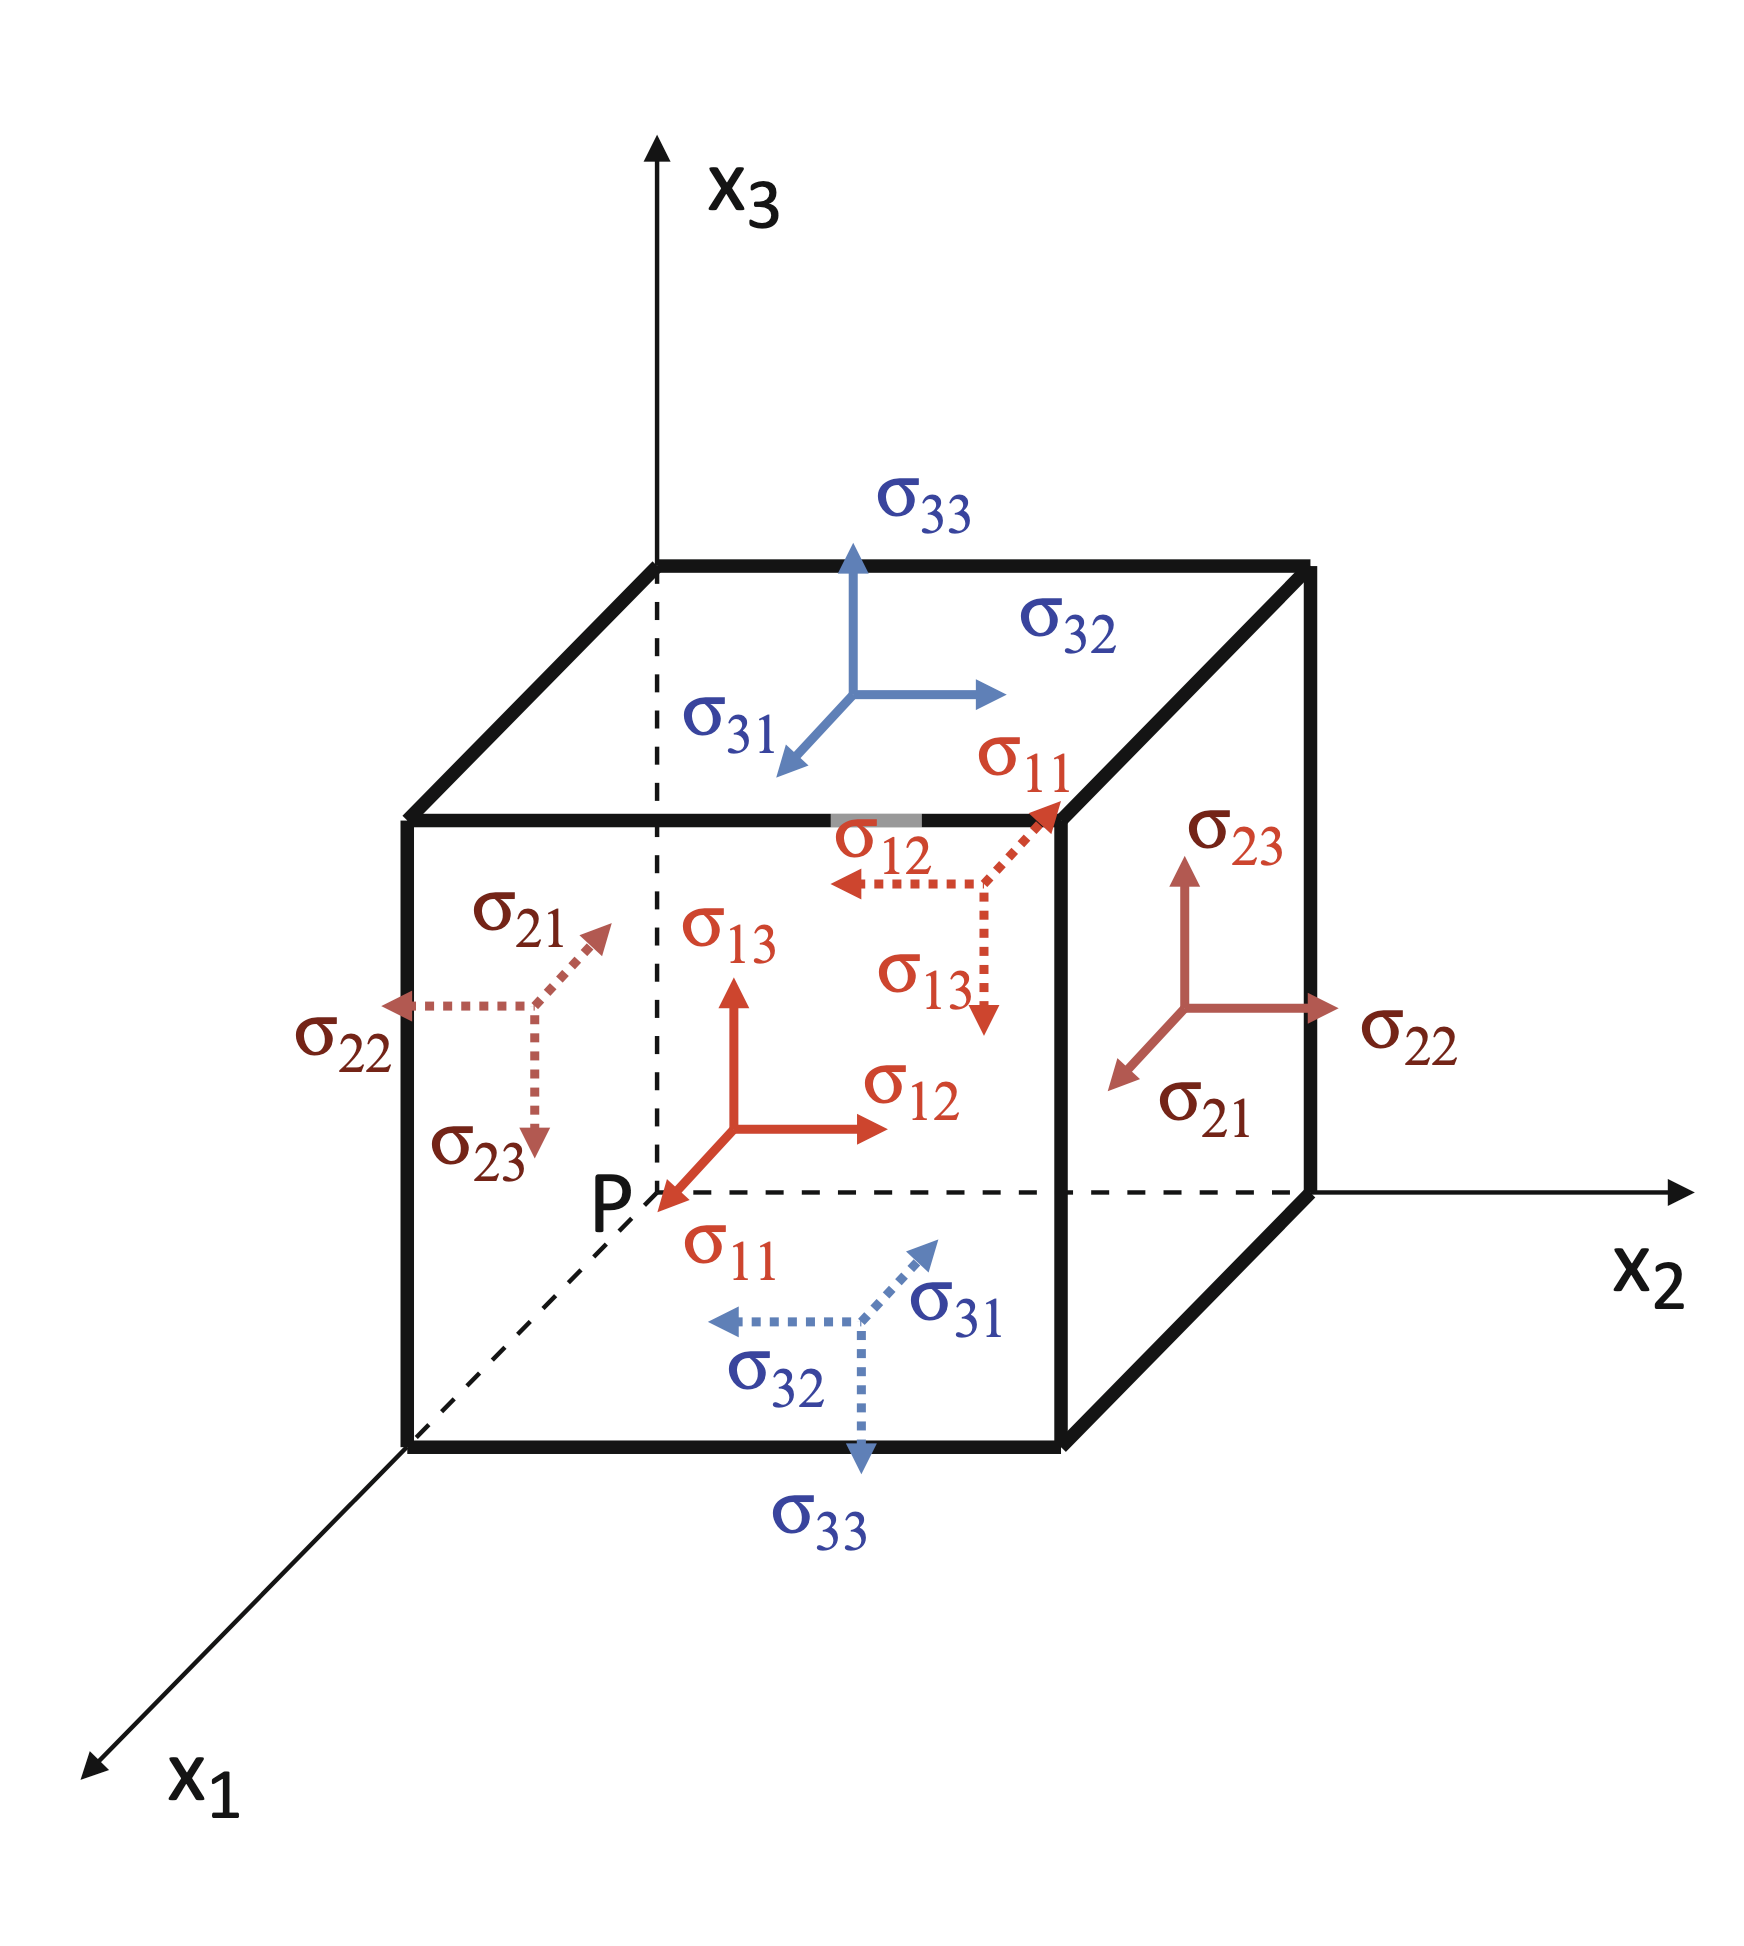
\includegraphics[width=2.5cm]{../images/stressComponents.png}

        \noindent{\tiny\emph{Credit: Neto et al.}}
      \end{center}
    \end{column}
    \hfill
    \begin{column}{.33\textwidth}
      \small\centering \textbf{Strain tensor}
      $$\boldsymbol{\varepsilon}(\mathbf x,t)=\begin{bmatrix}\varepsilon_{11}(\mathbf x,t)\\ \varepsilon_{22}(\mathbf x,t)\\ \varepsilon_{33}(\mathbf x,t)\\ 2\varepsilon_{23}(\mathbf x,t)\\ 2\varepsilon_{31}(\mathbf x,t)\\ 2\varepsilon_{12}(\mathbf x,t)\end{bmatrix}$$
    \end{column}
  \end{columns}
  \vspace{4pt}\noindent\color{darkred}\rule{\linewidth}{0.1mm}
  {\footnotesize
    \begin{block}{Generalised Hooke’s law}
      The constitutive stress-strain relationship of linear elasticity is given by the Hooke’s law:
      $$\boldsymbol\sigma(\mathbf x,t)       = \mathbf C\,\boldsymbol\varepsilon(\mathbf x,t)$$
      or equivalently
      $$\boldsymbol\varepsilon(\mathbf x,t)  = \mathbf S\, \boldsymbol\sigma(\mathbf x,t)$$
      where $\mathbf C$ is called the \emph{stiffness material matrix} and $\mathbf S=\mathbf C^{-1}$.
    \end{block}
  }
\end{frame}

\begin{frame}{Materials classification}
  \setlength{\arraycolsep}{2pt}
  \begin{columns}[t]
    \begin{column}{0.23\textwidth}
      \textbf{Anisotropic}
      \tiny $$\mathbf S=\begin{bmatrix} s_{11} & s_{12} & s_{13} & s_{14} & s_{15} & s_{16} \\ s_{21} & s_{22} & s_{23} & s_{24} & s_{25} & s_{26} \\ s_{31} & s_{32} & s_{33} & s_{34} & s_{35} & s_{36} \\ s_{41} & s_{42} & s_{43} & s_{44} & s_{45} & s_{46}\\ s_{51} & s_{52} & s_{53} & s_{54} & s_{55} & s_{56}\\ s_{61} & s_{62} & s_{63} & s_{64} & s_{65} & s_{66} \end{bmatrix}$$
      \begin{itemize}
        \item   have properties that vary with direction and do not have symmetry.
        \item 21 independent constants (symmetry).
      \end{itemize}
    \end{column}
    \begin{column}{0.33\textwidth}
      \textbf{Orthotropic}
      \tiny $$\mathbf S=\begin{bmatrix} \frac{1}{E_1} & -\frac{\nu_{21}}{E_2} & -\frac{\nu_{31}}{E_3} & 0 & 0 & 0 \\  -\frac{\nu_{12}}{E_1} & \frac{1}{E_2}  & -\frac{\nu_{32}}{E_3}  & 0 & 0 & 0 \\ -\frac{\nu_{13}}{E_1} & -\frac{\nu_{23}}{E_2} & \frac{1}{E_3} & 0 & 0 & 0 \\ 0 & 0 & 0 & \frac{1}{G_{23}} & 0 & 0 \\ 0 & 0 & 0 & 0 & \frac{1}{G_{31}} & 0 \\ 0 & 0 & 0 & 0 & 0 & \frac{1}{G_{12}} \end{bmatrix}$$
      \begin{itemize}
        \item Three planes of symmetry.
        \item $E_{i}$ is the Young's modulus.
        \item $G_{ij}$ is the shear modulus.
        \item $\nu_{ij}$ is the Poisson's ratio.
        \item 6 independent constants since:
              $$\frac{\nu_{12}}{E_1} = \frac{\nu_{21}}{E_2}, \
                \frac{\nu_{23}}{E_2} = \frac{\nu_{32}}{E_3}, \
                \frac{\nu_{31}}{E_3} = \frac{\nu_{13}}{E_1} $$
      \end{itemize}
    \end{column}
    \begin{column}{0.3\textwidth}
      \textbf{Isotropic}
      \tiny $$\mathbf S=\begin{bmatrix} 1/E & -\nu/E & -\nu/E & 0 & 0 & 0 \\  -\nu/E & 1/E  & -\nu/E  & 0 & 0 & 0 \\ -\nu/E & -\nu/E & 1/E & 0 & 0 & 0 \\ 0 & 0 & 0 & 1/G & 0 & 0 \\ 0 & 0 & 0 & 0 & 1/G & 0 \\ 0 & 0 & 0 & 0 & 0 & 1/G \end{bmatrix}$$
      \begin{itemize}
        \item Identical properties in all directions.
        \item $E$ is the Young's modulus, $G$ is the shear modulus, and $\nu$ is the Poisson's ratio.
        \item Only 2 independent constants since
              $$E=2G(1+\nu)$$
      \end{itemize}
    \end{column}
  \end{columns}
\end{frame}

\begin{frame}
  \frametitle{Strain-displacement relationship}
  \vspace{-.4cm}{\footnotesize\begin{itemize}
      \item Strain is obtained by derivatives of displacements for small deformations.
      \item The strain-displacement relation can be written in the \emph{three equivalent forms} as follows:
    \end{itemize}}
  \vspace{-.4cm}
  \begin{columns}[T]
    \hspace{1.5cm}\begin{column}{.5\textwidth}
      \begin{block}{Kinematics}
        \begin{enumerate}
          \item[a)] $\boldsymbol\varepsilon(\mathbf x,t) =\nabla\mathbf u(\mathbf x,t)$
                \vspace{0.2cm}
          \item[b)] $\begin{bmatrix}\varepsilon_{11}\\ \varepsilon_{22}\\ \varepsilon_{33}\\ 2\varepsilon_{23}\\ 2\varepsilon_{31}\\ 2\varepsilon_{12}\end{bmatrix}=\begin{bmatrix} \partial_x & 0 & 0 \\ 0 & \partial_y & 0 \\ 0 & 0 & \partial_z \\ 0 & \partial_z & \partial_y \\ \partial_z & 0 & \partial_x  \\ \partial_y & \partial_x & 0 \end{bmatrix}\begin{bmatrix}u_{1}\\ u_{2}\\ u_{3}\end{bmatrix}$
                \vspace{0.2cm}
          \item[c)] $\varepsilon_{ii}=\partial_{x_{i}}u_i$ and $2\varepsilon_{ij}=\partial_{x_{i}}u_j+\partial_{x_{j}}u_i$
        \end{enumerate}
      \end{block}
    \end{column}
  \end{columns}
\end{frame}



{\setbeamercolor{background canvas}{bg=darkred}
\setbeamercolor{block body}{bg=darkred,fg=white}
\setbeamercolor{itemize item}{fg=white}
\begin{frame}{Differential equations of motion a.k.a equilibrium equations}
  \begin{block}{}
    \begin{itemize}
      \item The equilibrium equation of elastodynamics in matrix form is:
            $$\nabla^T\boldsymbol\sigma(\mathbf x,t)+\mathbf f(\mathbf x,t)=\rho\, \mathbf{\ddot{u}}(\mathbf x,t)$$
      \item Using the strain-displacement relation we can write it in terms of the displacement filed:
            $$\nabla^T\mathbf C\nabla\mathbf u(\mathbf x,t)+\mathbf f(\mathbf x,t)=\rho\, \mathbf{\ddot{u}}(\mathbf x,t)$$
    \end{itemize}
  \end{block}
\end{frame}
}

{\setbeamercolor{background canvas}{bg=darkred}
\setbeamercolor{block body}{bg=darkred,fg=white}
\setbeamercolor{itemize item}{fg=white}
\begin{frame}{Strong form of elastodynamics}
  \begin{block}{}
    Given a deformable solid $\Omega$ with boundary $\Gamma$, and
    \begin{itemize}
      \item stiffness material matrix $\mathbf C$ and material density $\rho$,
      \item prescribed body load $\mathbf f$ applied on $\Omega$,
      \item prescribed boundary displacement $\mathbf{\hat u}$ on $\Gamma_{u}$ and surface load $\mathbf{\hat f}$ on $\Gamma_{\sigma}$,
      \item prescribed initial (at $t=0$) displacement $\mathbf u_{0}$ and initial velocity $\mathbf v_{0}$,
    \end{itemize}
    \begin{columns}[T]
      \begin{column}{.6\textwidth}
        find the displacement $\mathbf u\in C^{2}(\bar\Omega\times[0,T],\mathbb R^{3})$ such that
        $$\begin{cases}
            \nabla^T\mathbf C\nabla \mathbf u+\mathbf f=\rho\, \mathbf{\ddot{u}} & \text{on }\Omega\times]0,T[         \\
            \mathbf u=\mathbf{\hat u}                                            & \text{on } \Gamma_u\times]0,T[      \\
            \mathbf N^T\mathbf  C\nabla\mathbf  u=\mathbf{\hat f}                & \text{on } \Gamma_\sigma\times]0,T[ \\
            \mathbf u=\mathbf u_0                                                & \text{for } t=0                     \\
            \mathbf{\dot u} =\mathbf v_0                                         & \text{for } t=0                     \\
          \end{cases}$$
      \end{column}
      \hfill
      \begin{column}{.2\textwidth}
        \vspace{-0.5cm}
        \begin{center}
          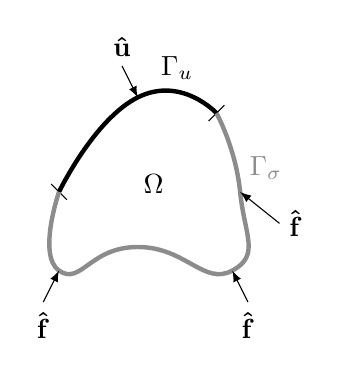
\begin{tikzpicture}
            % Label the region Omega	
            \node at (2.2,2.1) {$\Omega$};
            % Label the boundary Gamma
            \draw[ultra thick] plot [smooth, tension=1] coordinates {(1,2) (2,3.2) (3,3)};
            \node[above] at (2.5,3.3) {$\Gamma_u$};
            \draw[thin] (3+0.1,3+0.1) --(3-0.1,3-0.1);
            \draw[thin] (1+0.1,2-0.1) --(1-0.1,2+0.1);
            \draw[latex-]  (2,3.2) --  (2-0.2,3.2+0.4) node[above] {$\mathbf{\hat u}$};
            % Draw part of the boundary Gamma_sigma
            \draw[ultra thick, gray!90] plot [smooth, tension=1] coordinates {(3,3) (3.3,2) (3.2,1) (2,1.3) (1,1) (1,2)};
            \node[gray!90, right] at (3.3,2.3) {$\Gamma_\sigma$};
            \draw[latex-]  (1,1) --  (1-0.2,1-0.4) node[below] {$\mathbf{\hat f}$};;
            \draw[latex-]  (3.2,1) --  (3.2+0.2,1-0.4) node[below] {$\mathbf{\hat f}$};
            \draw[latex-]  (3.3,2) --  (3.3+0.5,2-0.4) node[right] {$\mathbf{\hat f}$};
          \end{tikzpicture}
        \end{center}
      \end{column}
    \end{columns}

  \end{block}
\end{frame}
}


\begin{frame}{Strong and weak forms of elastodynamics}
  \vspace{-0.5cm}
  \begin{center}
    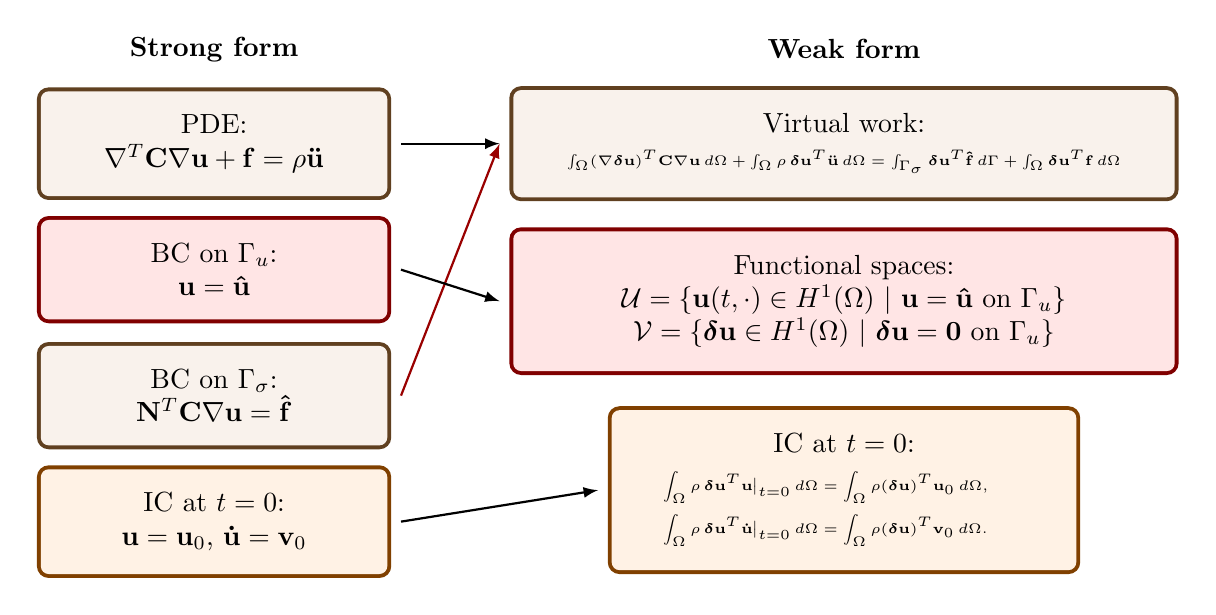
\begin{tikzpicture}[scale=0.8]
      \node (sf) at (-2,6.5) {
        \centering \textbf{Strong form}
      };
      \node (wf) at (8,6.5) {
        \centering \textbf{Weak form}
      };
      \node (pde) at (-2,5) {
        \begin{tcolorbox}[colframe=brown!50!black, colback=brown!10, coltitle=black, rounded corners, width=4.5cm]
          \centering PDE: \\ $\nabla^T\mathbf C\nabla \mathbf u+\mathbf f=\rho\mathbf{\ddot{u}}$
        \end{tcolorbox}
      };
      \node (bc1) at (-2,3) {
        \begin{tcolorbox}[colframe=red!50!black, colback=red!10, coltitle=black, rounded corners,width=4.5cm]
          \centering BC on $\Gamma_u$: \\ $\mathbf u=\mathbf{\hat u}$
        \end{tcolorbox}
      };
      \node (bc2) at (-2,1) {
        \begin{tcolorbox}[colframe=brown!50!black, colback=brown!10, coltitle=black, rounded corners,width=4.5cm]
          \centering BC on $\Gamma_\sigma$: \\ $\mathbf N^T\mathbf  C\nabla\mathbf  u=\mathbf{\hat f}$
        \end{tcolorbox}
      };

      \node (ic1) at (-2,-1) {
        \begin{tcolorbox}[colframe=orange!50!black, colback=orange!10, coltitle=black, rounded corners,width=4.5cm]
          \centering IC at $t=0$: \\ $\mathbf{u}=\mathbf u_0$, $\mathbf{\dot u}=\mathbf v_0$
        \end{tcolorbox}
      };
      \node (inteq) at (8,5) {
        \begin{tcolorbox}[colframe=brown!50!black, colback=brown!10, coltitle=black, rounded corners, width=8.5cm]
          \centering Virtual work: \\\vspace{0.2cm} \tiny $\int_\Omega (\nabla \bolddelta\mathbf u)^{T} \mathbf C\nabla \mathbf u\, d\Omega+\int_\Omega\rho\, \bolddelta\mathbf u^{T}\mathbf{\ddot{u}}\, d\Omega=\int_{\Gamma_\sigma} \bolddelta\mathbf u^{T}\mathbf{\hat f} \, d\Gamma+\int_\Omega \bolddelta\mathbf u^{T}\mathbf f\, d\Omega$
        \end{tcolorbox}
      };
      \node (funcsp) at (8,2.5) {
        \begin{tcolorbox}[colframe=red!50!black, colback=red!10, coltitle=black, rounded corners,width=8.5cm]
          \centering Functional spaces: \\ $ \mathcal U =\{\mathbf u(t,\cdot)\in H^1(\Omega)\ |\ \mathbf u=\mathbf{\hat u}\ \mbox{on}\ \Gamma_u\}$ \\
          $ \mathcal V =\{\bolddelta\mathbf u\in H^1(\Omega)\ |\ \bolddelta\mathbf u=\mathbf 0\ \mbox{on}\ \Gamma_u\}$
        \end{tcolorbox}
      };
      \node (ic2) at (8,-0.5) {
        \begin{tcolorbox}[colframe=orange!50!black, colback=orange!10, coltitle=black, rounded corners,width=6cm]
          \centering IC at $t=0$: \\ \vspace{0.2cm} \tiny $\begin{aligned}
               & \int_{\Omega}\rho\, \bolddelta\mathbf u^{T}\mathbf u\big |_{t=0}\, d\Omega =\int_{\Omega}\rho (\bolddelta\mathbf u)^{T}\mathbf u_0\, d\Omega,\hspace{0.5cm} \\
               & \int_{\Omega}\rho\, \bolddelta\mathbf u^{T}\mathbf{\dot u}\big |_{t=0}\, d\Omega =\int_{\Omega}\rho (\bolddelta\mathbf u)^{T}\mathbf v_0\, d\Omega.
            \end{aligned}$
        \end{tcolorbox}
      };
      % Drawing arrows
      \draw[-latex, thick] (pde.east) -- (inteq.west);
      \draw[-latex, thick, darkred] (bc2.east) -- (inteq.west);
      \draw[-latex, thick] (bc1.east) -- (funcsp.west);
      \draw[-latex, thick] (ic1.east) -- (ic2.west);
    \end{tikzpicture}
  \end{center}
\end{frame}

\begin{frame}{Weighted residuals}
  \begin{itemize}
    \item  Let $\mathbf u$ be a solution of
          $$\nabla^T\mathbf C\nabla \mathbf u+\mathbf f-\rho\mathbf{\ddot{u}}=0.$$
    \item Let $\mathbf u^{h}$ an approximate solution.
          \begin{block}{}
            In general $\mathbf u^{h}$ does not satisfy the differential equation and hence results in an error or a \emph{residual}:
            $$\nabla^T\mathbf C\nabla \mathbf u^{h}+\mathbf f-\rho\mathbf{\ddot{u}}^{h}=\mathbf R^{h}.$$
          \end{block}
    \item We impose that the residual is zero in a certain Euclidean vector space $\mathcal V^h$ of finite dimension. Thus
          $$\langle\mathbf R^{h}, \mathbf v^h\rangle=0\qquad \text{for all }\mathbf v^h\in\mathcal V^{h}$$
          where $\langle\cdot,\cdot\rangle$ denotes the scalar product.
  \end{itemize}
\end{frame}


\section{Discretization and Galerkin method}

\begin{frame}{General ideas of Galerkin methods}
  \begin{columns}[T]
    \begin{column}{.68\textwidth}\vspace{1.2cm}
      \vspace{-1cm}
      \begin{center}
        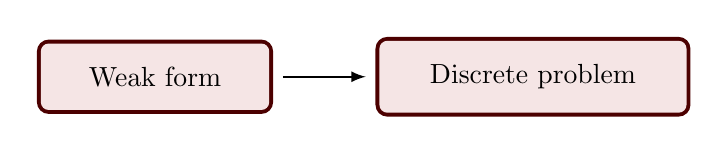
\begin{tikzpicture}[scale=0.8]
          \node (wr) at (-2,0) {
            \begin{tcolorbox}[colframe=darkred!50!black, colback=darkred!10, coltitle=black, rounded corners, width=3cm]
              \centering Weak form
            \end{tcolorbox}
          };
          \node (dp) at (4,0) {
            \begin{tcolorbox}[colframe=darkred!50!black, colback=darkred!10, coltitle=black, rounded corners, width=4cm]
              \centering Discrete problem
            \end{tcolorbox}
          };
          % Drawing arrows
          \draw[-latex, thick] (wr.east) -- (dp.west);
        \end{tikzpicture}
      \end{center}

      \begin{itemize}
        \item Galerkin methods are a class of numerical techniques used to transform differential equations in weak formulation, into discrete problems.
        \item The approximate solution is determined via a finite set of \textbf{basis functions}.
        \item Galerkin approximation compute the best possible approximate solution among a family of potential solutions.
      \end{itemize}

    \end{column}
    \hfill
    \begin{column}{.28\textwidth}
      \begin{center}
        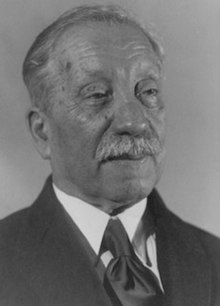
\includegraphics[scale=0.5]{../images/Galerkin}

        \noindent{\tiny\emph{Boris Galerkin 1871 - 1945}}
      \end{center}
    \end{column}
  \end{columns}
\end{frame}

\begin{frame}{Approximate solution of the weak form}
  Choose subspaces $\mathcal U^{h}\subset \mathcal U$ and $\mathcal V^{h}\subset \mathcal V$ of {\color{darkred}dimension $n$}  and solve the \emph{projected weak form} into such subspaces. Moreover, we impose $\mathcal U^{h}=\mathcal V^{h}$.
  \vspace{0.1cm}
  \begin{block}{\large Displacement approximation}
    Let $\mathbf u^{h}(\mathbf x,t)=\mathbf H(\mathbf x)\mathbf q(t)$ and $\bolddelta\mathbf u^{h}(\mathbf x)=\mathbf H(\mathbf x)\bolddelta\mathbf q$ where
    \begin{itemize}
      \item $\mathbf H(\mathbf x)$ is a $3\times n$ matrix of l.i. \textbf{shape functions} (basis of $\mathcal U^h=\mathcal V^h$).
      \item $\mathbf q(t)$ is a $n\times 1$ vector of (\emph{unknown}) time-dependent functions.
      \item $\bolddelta \mathbf q$ is a $n\times 1$ vector of constants.
    \end{itemize}
    \vspace{0.5cm}
    $$\mathbf u^{h}(\mathbf x,t)=\mathbf H(\mathbf x)\mathbf q(t)\qquad\text{and}\qquad \delta\mathbf u^{h}(\mathbf x)=\mathbf H(\mathbf x)\delta\mathbf q.$$
  \end{block}
\end{frame}

\begin{frame}{Formulations of elastodynamics}
  \vspace{-0.5cm}
  \begin{center}
    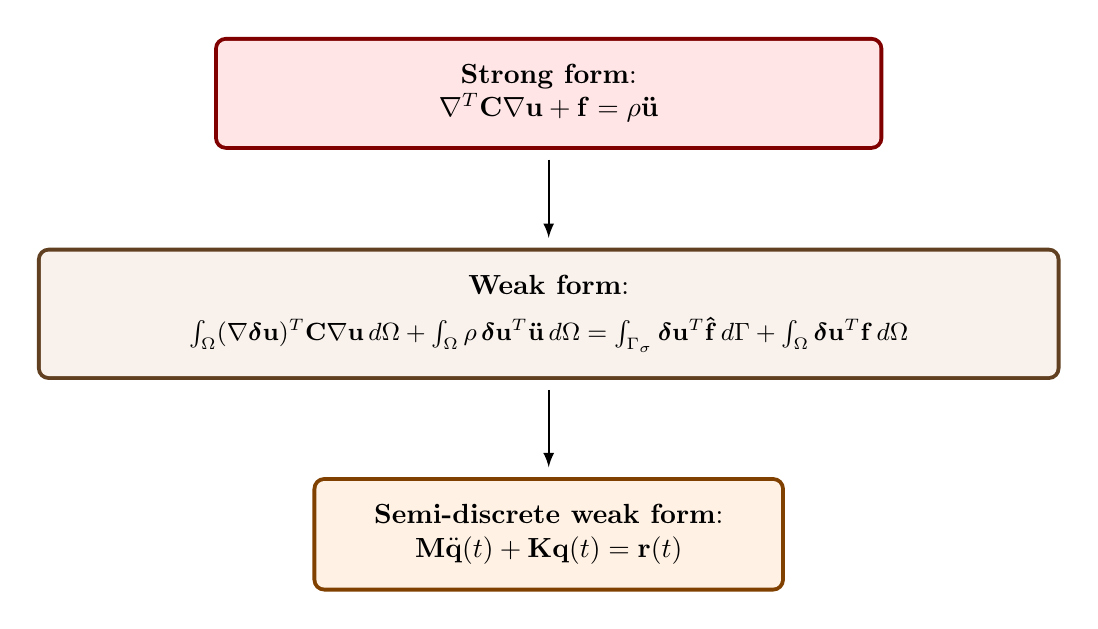
\begin{tikzpicture}[scale=0.7]
      \node (sf) at (0,6) {
        \begin{tcolorbox}[colframe=red!50!black, colback=red!10, coltitle=black, rounded corners,width=8.5cm]
          \centering \textbf{Strong form}: \\ $\nabla^T\mathbf C\nabla \mathbf u+\mathbf f=\rho\mathbf{\ddot{u}}$
        \end{tcolorbox}
      };
      \node (wf) at (0,2) {
        \begin{tcolorbox}[colframe=brown!50!black, colback=brown!10, coltitle=black, rounded corners, width=13cm]
          \centering \textbf{Weak form}: \\\vspace{0.2cm} \small $\int_\Omega (\nabla \bolddelta\mathbf u)^{T} \mathbf C\nabla \mathbf u\, d\Omega+\int_\Omega\rho\, \bolddelta\mathbf u^{T}\mathbf{\ddot{u}}\, d\Omega=\int_{\Gamma_\sigma} \bolddelta\mathbf u^{T}\mathbf{\hat f} \, d\Gamma+\int_\Omega \bolddelta\mathbf u^{T}\mathbf f\, d\Omega$
        \end{tcolorbox}
      };
      \node (sdwf) at (0,-2) {
        \begin{tcolorbox}[colframe=orange!50!black, colback=orange!10, coltitle=black, rounded corners,width=6cm]
          \centering \textbf{Semi-discrete weak form}: \\ $\mathbf M\ddot{\mathbf q}(t)+\mathbf K\mathbf q(t)=\mathbf r(t)$
        \end{tcolorbox}
      };
      % Drawing arrows
      \draw[-latex, thick] (sf.south) -- (wf.north);
      \draw[-latex, thick] (wf.south) -- (sdwf.north);
    \end{tikzpicture}
  \end{center}
\end{frame}

\begin{frame}{Definitions}
  \begin{block}{}
    \begin{itemize}
      \item \textbf{Stiffness matrix} ($n\times n$):
            $$\mathbf K=\int_\Omega \mathbf B^T\mathbf C\mathbf B \, d\Omega$$
            where $\mathbf B$ is the ($6\times n$) deformation matrix defined by $\mathbf B=\nabla \mathbf H$.
      \item \textbf{Mass matrix} ($n\times n$):
            $$\mathbf M=\int_\Omega \rho\, \mathbf H^T\mathbf H \, d\Omega.$$
      \item \textbf{Applied forces vector} ($n\times 1$):
            $$\mathbf r(t)=\int_{\Gamma_\sigma} \mathbf H^{T}\mathbf{\hat f} \, d\Gamma+\int_{\Omega} \mathbf H^{T}\mathbf f\, d\Omega.$$
    \end{itemize}
  \end{block}
\end{frame}

\section{Finite element method}

\begin{frame}{Divide and conquer mentality}
  \textbf{Finite element method:} a special case of the Galerkin method, where shape functions are systematically defined in terms of nodes.
  \vspace{-0.6cm}
  \begin{columns}
    \begin{column}{0.3\textwidth}
      \begin{center}
        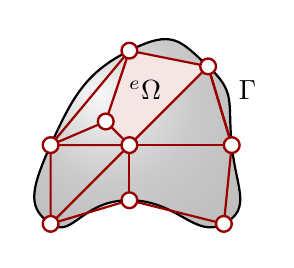
\begin{tikzpicture}[scale=1]
          %\draw[step=1.0,black,thin] (0,0) grid (4,4);
          % Draw the potato-like shape
          \shade [ball color= gray!90!black, opacity=.3] plot [thick,smooth cycle, tension=1] coordinates  {(1,2) (2,3.2) (3,3) (3.3,2) (3.2,1) (2,1.3) (1,1)};
          \draw[thick] plot [thick,smooth cycle, tension=1] coordinates {(1,2) (2,3.2) (3,3) (3.3,2) (3.2,1) (2,1.3) (1,1)};
          \draw[fill=darkred!30,thick,darkred!10] (2,2) -- (3,3) -- (2,3.2) -- (1.7,2.3) -- cycle;
          % Label the region Omega	
          \node at (2.2,2.7) {${}^e\Omega$};
          % Label the boundary Gamma
          \node at (3.5,2.7) {$\Gamma$};
          \draw[thick,darkred] (1,2) -- (2,3.2) -- (3,3) -- (3.3,2) -- (3.2,1) -- (2,1.3) -- (1,1) -- cycle;
          \draw[thick,darkred] (1,2) -- (2,2) -- (3,3) -- (3.3,2);
          \draw[thick,darkred] (2,1.3) -- (2,2) -- (3.3,2);
          \draw[thick,darkred] (1,1) -- (2,2) -- (1.7,2.3) -- (2,3.2);
          \draw[thick,darkred] (1.7,2.3) -- (1,2);
          \node[darkred,draw,shape=circle,fill=white,minimum size=2mm,line width=0.3mm,inner sep=0] at (1,1) {};
          \node[darkred,draw,shape=circle,fill=white,minimum size=2mm,line width=0.3mm,inner sep=0] at (1,2) {};
          \node[darkred,draw,shape=circle,fill=white,minimum size=2mm,line width=0.3mm,inner sep=0] at (2,2) {};
          \node[darkred,draw,shape=circle,fill=white,minimum size=2mm,line width=0.3mm,inner sep=0] at (2,1.3) {};
          \node[darkred,draw,shape=circle,fill=white,minimum size=2mm,line width=0.3mm,inner sep=0] at (2,3.2) {};
          \node[darkred,draw,shape=circle,fill=white,minimum size=2mm,line width=0.3mm,inner sep=0] at (1.7,2.3) {};
          \node[darkred,draw,shape=circle,fill=white,minimum size=2mm,line width=0.3mm,inner sep=0] at (3,3) {};
          \node[darkred,draw,shape=circle,fill=white,minimum size=2mm,line width=0.3mm,inner sep=0] at (3.2,1) {};
          \node[darkred,draw,shape=circle,fill=white,minimum size=2mm,line width=0.3mm,inner sep=0] at (3.3,2) {};
        \end{tikzpicture}
      \end{center}
    \end{column}
    \begin{column}{0.5\textwidth}
      \begin{center}
        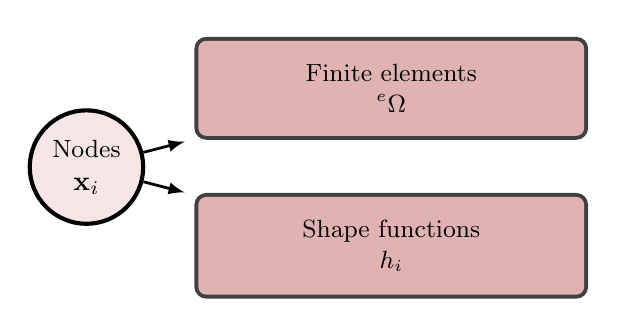
\begin{tikzpicture}[scale=0.5, node distance=0.5cm,>=stealth,thick]
          % Define nodes
          \node (Nodes) [circle, draw, minimum size=1cm, align=center, fill=darkred!10,line width=1.5pt] {\small Nodes\\ $\mathbf x_i$};

          \node (Elem) [right=of Nodes, yshift=+1cm]  {
            \begin{tcolorbox}[colback=darkred!30, width=5cm]
              \small \centering Finite elements \\ $\mathbf {}^e\Omega$
            \end{tcolorbox}
          };

          \node (Func) [right=of Nodes, yshift=-1cm]  {
            \begin{tcolorbox}[colback=darkred!30, width=5cm]
              \small \centering Shape functions\\ $h_i$
            \end{tcolorbox}
          };

          % Draw arrows
          \draw[-latex,line width=1pt] (Nodes) -- (Elem);
          \draw[-latex,line width=1pt] (Nodes) -- (Func);
        \end{tikzpicture}
      \end{center}
    \end{column}
  \end{columns}
  \begin{itemize}
    \item The geometry of a structure is discretised when it is split into a mesh of finite elements ${}^1\Omega,\dots,{}^m\Omega$ (smaller components or regular shapes).
    \item Each shape function is non-zero only on a very limited number of finite elements (\emph{compact support}).
  \end{itemize}
\end{frame}

\begin{frame}{Displacements approximation in finte element method}
  \vspace{-1cm}
  \begin{columns}[T]
    \begin{column}{.4\textwidth}
      \begin{center}
        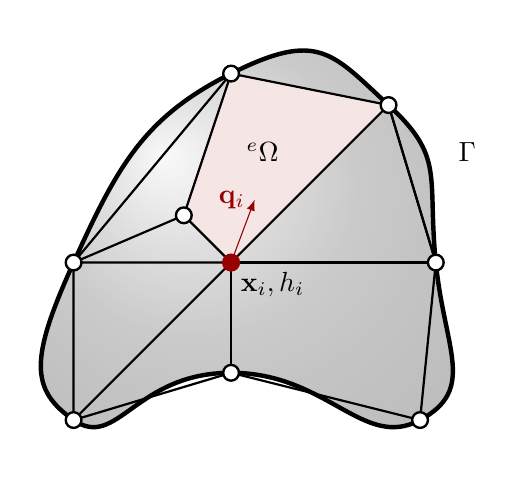
\begin{tikzpicture}[scale=2]
          %\draw[step=1.0,black,thin] (0,0) grid (4,4);
          % Draw the potato-like shape
          \shade [ball color= gray!90!black, opacity=.3] plot [thick,smooth cycle, tension=1] coordinates  {(1,2) (2,3.2) (3,3) (3.3,2) (3.2,1) (2,1.3) (1,1)};
          \draw[ultra thick] plot [thick,smooth cycle, tension=1] coordinates {(1,2) (2,3.2) (3,3) (3.3,2) (3.2,1) (2,1.3) (1,1)};
          \draw[fill=darkred!30,thick,darkred!10] (2,2) -- (3,3) -- (2,3.2) -- (1.7,2.3) -- cycle;
          \node[below right] at (2,2) {$\mathbf x_i, h_i$};
          \draw[-latex,darkred] (2,2) -- (2.15,2.4) node[darkred, left]{$\mathbf q_i$};
          % Label the region Omega	
          \node at (2.2,2.7) {${}^e\Omega$};
          % Label the boundary Gamma
          \node at (3.5,2.7) {$\Gamma$};
          \draw[thick] (1,2) -- (2,3.2) -- (3,3) -- (3.3,2) -- (3.2,1) -- (2,1.3) -- (1,1) -- cycle;
          \draw[thick] (1,2) -- (2,2) -- (3,3) -- (3.3,2);
          \draw[thick] (2,1.3) -- (2,2) -- (3.3,2);
          \draw[thick] (1,1) -- (2,2) -- (1.7,2.3) -- (2,3.2);
          \draw[thick] (1.7,2.3) -- (1,2);
          \node[darkred,draw,shape=circle,fill=darkred,minimum size=2mm,line width=0.3mm,inner sep=0] at (2,2) {};
          \node[draw,shape=circle,fill=white,minimum size=2mm,line width=0.3mm,inner sep=0] at (1,1) {};
          \node[draw,shape=circle,fill=white,minimum size=2mm,line width=0.3mm,inner sep=0] at (1,2) {};
          \node[draw,shape=circle,fill=white,minimum size=2mm,line width=0.3mm,inner sep=0] at (2,1.3) {};
          \node[draw,shape=circle,fill=white,minimum size=2mm,line width=0.3mm,inner sep=0] at (2,3.2) {};
          \node[draw,shape=circle,fill=white,minimum size=2mm,line width=0.3mm,inner sep=0] at (1.7,2.3) {};
          \node[draw,shape=circle,fill=white,minimum size=2mm,line width=0.3mm,inner sep=0] at (3,3) {};
          \node[draw,shape=circle,fill=white,minimum size=2mm,line width=0.3mm,inner sep=0] at (3.2,1) {};
          \node[draw,shape=circle,fill=white,minimum size=2mm,line width=0.3mm,inner sep=0] at (3.3,2) {};
        \end{tikzpicture}
      \end{center}
    \end{column}
    \begin{column}{.6\textwidth}
      Let $p$ the number of nodes of the mesh.
      \vspace{-.2cm}
      \begin{align*}
        \mathbf u^{h}(\mathbf x,t) & =\mathbf H(\mathbf x)\mathbf q(t) = \sum_{i=1}^{p}h_{i}(\mathbf x)\mathbf q_{i}(t)
      \end{align*}
      \vspace{-.5cm}
      \begin{itemize}
        \item $\mathbf H(\mathbf x)$ is a $3\times 3p$ matrix of \textbf{shape functions}:
              $$
                \mathbf H
                =\left[
                  \begin{array}{c;{2pt/2pt}c;{2pt/2pt}c;{2pt/2pt}c;{2pt/2pt}c;{2pt/2pt}c}
                    h_{1}\mathbf I & h_{2}\mathbf I & \dots & h_{i}\mathbf I & \dots & h_{p}\mathbf I \\
                  \end{array} \right]
              $$
              $\mathbf I$ is the $3\times 3$ identity matrix.
        \item $\mathbf q(t)$ is a $3p\times 1$ vector of (\emph{unknown}) nodal displacements.

      \end{itemize}
    \end{column}
  \end{columns}
\end{frame}


\begin{frame}{Global nodal shape functions requirements}
  \vspace{-1cm}
  \begin{columns}[T]
    \begin{column}{.4\textwidth}
      \begin{center}
        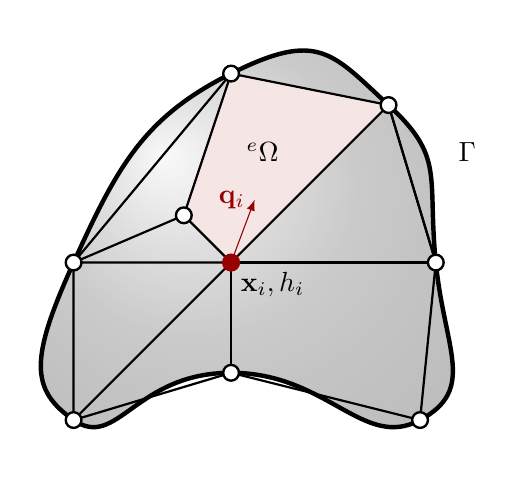
\begin{tikzpicture}[scale=2]
          %\draw[step=1.0,black,thin] (0,0) grid (4,4);
          % Draw the potato-like shape
          \shade [ball color= gray!90!black, opacity=.3] plot [thick,smooth cycle, tension=1] coordinates  {(1,2) (2,3.2) (3,3) (3.3,2) (3.2,1) (2,1.3) (1,1)};
          \draw[ultra thick] plot [thick,smooth cycle, tension=1] coordinates {(1,2) (2,3.2) (3,3) (3.3,2) (3.2,1) (2,1.3) (1,1)};
          \draw[fill=darkred!30,thick,darkred!10] (2,2) -- (3,3) -- (2,3.2) -- (1.7,2.3) -- cycle;
          \node[below right] at (2,2) {$\mathbf x_i, h_i$};
          \draw[-latex,darkred] (2,2) -- (2.15,2.4) node[darkred, left]{$\mathbf q_i$};
          % Label the region Omega	
          \node at (2.2,2.7) {${}^e\Omega$};
          % Label the boundary Gamma
          \node at (3.5,2.7) {$\Gamma$};
          \draw[thick] (1,2) -- (2,3.2) -- (3,3) -- (3.3,2) -- (3.2,1) -- (2,1.3) -- (1,1) -- cycle;
          \draw[thick] (1,2) -- (2,2) -- (3,3) -- (3.3,2);
          \draw[thick] (2,1.3) -- (2,2) -- (3.3,2);
          \draw[thick] (1,1) -- (2,2) -- (1.7,2.3) -- (2,3.2);
          \draw[thick] (1.7,2.3) -- (1,2);
          \node[darkred,draw,shape=circle,fill=darkred,minimum size=2mm,line width=0.3mm,inner sep=0] at (2,2) {};
          \node[draw,shape=circle,fill=white,minimum size=2mm,line width=0.3mm,inner sep=0] at (1,1) {};
          \node[draw,shape=circle,fill=white,minimum size=2mm,line width=0.3mm,inner sep=0] at (1,2) {};
          \node[draw,shape=circle,fill=white,minimum size=2mm,line width=0.3mm,inner sep=0] at (2,1.3) {};
          \node[draw,shape=circle,fill=white,minimum size=2mm,line width=0.3mm,inner sep=0] at (2,3.2) {};
          \node[draw,shape=circle,fill=white,minimum size=2mm,line width=0.3mm,inner sep=0] at (1.7,2.3) {};
          \node[draw,shape=circle,fill=white,minimum size=2mm,line width=0.3mm,inner sep=0] at (3,3) {};
          \node[draw,shape=circle,fill=white,minimum size=2mm,line width=0.3mm,inner sep=0] at (3.2,1) {};
          \node[draw,shape=circle,fill=white,minimum size=2mm,line width=0.3mm,inner sep=0] at (3.3,2) {};
        \end{tikzpicture}
      \end{center}
    \end{column}
    \begin{column}{.6\textwidth}
      \textbf{Propretries of $h_i$:}
      \begin{itemize}
        \item Linearly independent polynomial basis.
        \item Satisfy Kronecker delta property:
              $$ h_i(\mathbf{x}_i) = 1\quad\text{and} \quad h_i(\mathbf{x}_j) = 0.$$
        \item Vanish on non-adjacent elements.
        \item Continuous at interfaces.
        \item Differentiable inside elements.
        \item Ensure rigid body motion \& constant deformations.
      \end{itemize}
    \end{column}
  \end{columns}
\end{frame}



\begin{frame}{Bilinear triangular shape functions}
  \begin{center}
    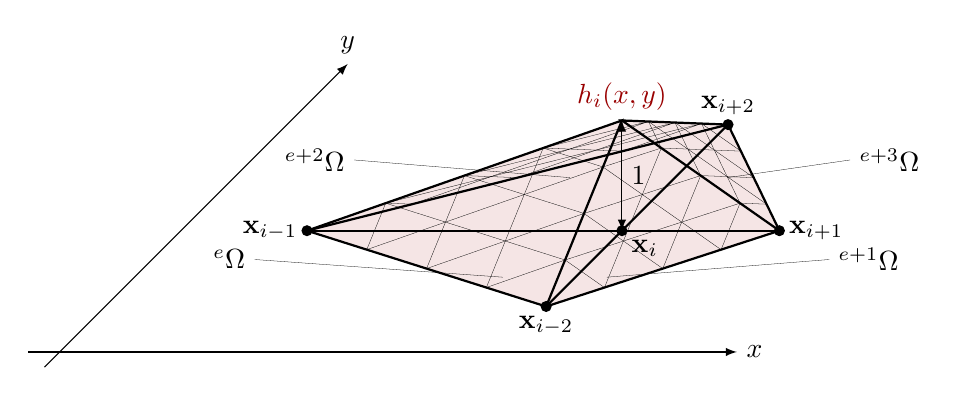
\begin{tikzpicture}
      \def\a{4}
      \def\b{3.5}
      \def\c{6}
      \def\h{1.4},
      \coordinate (x2) at (\a,0, 0);
      \coordinate (x4) at (0,0, \b);
      \coordinate (x5) at (\a,0, \b);
      \coordinate (x51) at (\a,\h, \b);
      \coordinate (x6) at (\c,0, \b);
      \coordinate (x8) at (\a,0, \c);
      %Color fill
      \filldraw[darkred!10] (x2) -- (x51) -- (x4) -- cycle;
      \filldraw[darkred!10] (x2) -- (x51) -- (x6) -- cycle;
      \filldraw[darkred!10] (x4) -- (x51) -- (x8) -- cycle;
      \filldraw[darkred!10] (x51) -- (x6) -- (x8) -- cycle;
      %Draw labels
      \fill (x2) circle (2pt) node[above] {$\mathbf x_{i+2}$};
      \fill (x4) circle (2pt) node[left] {$\mathbf x_{i-1}$};
      \fill (x5) circle (2pt) node[below right] {$\mathbf x_{i}$};
      \fill (x6) circle (2pt) node[right] {$\mathbf x_{i+1}$};
      \fill (x8) circle (2pt) node[below] {$\mathbf x_{i-2}$};
      \draw[ultra thin] (\a/1.5,0,\b/2) -- (-0.3,0,\b/3) node[left] {${}^{e+2}\Omega$};
      \draw[ultra thin] (\a/1.3,0,2.6*\b/3+\c/3) -- (-0.3,0,2.6*\b/3+\c/3-\b/6) node[left] {${}^{e}\Omega$};
      \draw[ultra thin] (2*\a/3+\c/3,0,\b/2) -- (\c,0,\b/3)node[right] {${}^{e+3}\Omega$};
      \draw[ultra thin] (1.8*\a/3+\c/3,0,2.6*\b/3+\c/3) -- (\c+1,0,2.6*\b/3+\c/3-\b/6)node[right] {${}^{e+1}\Omega$};
      %Draw lines
      \draw[thick] (x2) -- (x6) -- (x8) -- (x4) -- cycle;
      \draw[thick] (x2) -- (x5) -- (x8);
      \draw[thick] (x4) -- (x5) -- (x6);
      \draw[latex-latex] (x5) -- (x51) node[midway,right] {$1$} node[above]{{\color{darkred}$h_i(x,y)$}};
      \draw[thick] (x2) -- (x51) -- (x6);
      \draw[thick] (x4) -- (x51) -- (x8);
      %draw thin lines
      \foreach \i in {1,2,3} {
          \pgfmathsetmacro{\t}{\i/4} % Normalize parameter (dividing into 5 segments)
          \pgfmathsetmacro{\x}{(1-\t)*\a} % Linear interpolation for x
          \pgfmathsetmacro{\xb}{\t*\a} % Linear interpolation for x
          \pgfmathsetmacro{\z}{\t*\b}
          \pgfmathsetmacro{\y}{\t*\h} % Linear interpolation for y
          \coordinate (P\i) at (\x, 0, \z);
          \coordinate (Q\i) at (\a, \y, \z);
          \coordinate (R\i) at (\xb, \y, \b);
        }
      \foreach \i in {1, 2, 3} { % Generate 3 equidistant points
          \pgfmathsetmacro{\t}{\i/4} % Normalize the parameter (divide by 4 for 3 points)
          \pgfmathsetmacro{\x}{\t*\a} % Interpolate x-coordinate
          \pgfmathsetmacro{\z}{(1-\t)*\b + \t*\c} % Interpolate z-coordinate
          \coordinate (S\i) at (\x,0, \z); % Define the equidistant point
        }
      \foreach \i in {1, 2, 3} { % Generate 3 equidistant points
          \pgfmathsetmacro{\t}{\i/4} % Normalize the parameter (divide by 4 for 3 points)
          \pgfmathsetmacro{\x}{(1-\t)*\a + \t*\c} % Interpolate x-coordinate
          \pgfmathsetmacro{\z}{(1-\t)*\c + \t*\b} % Interpolate z-coordinate
          \coordinate (T\i) at (\x,0,\z); % Define the equidistant point
        }
      \foreach \i in {1, 2, 3} { % Generate 3 equidistant points
          \pgfmathsetmacro{\t}{\i/4} % Normalize the parameter (divide by 4 for 3 points)
          \pgfmathsetmacro{\x}{(1-\t)*\a + \t*\c} % Interpolate x-coordinate
          \pgfmathsetmacro{\z}{\t*\b} % Interpolate z-coordinate
          \coordinate (U\i) at (\x,0, \z); % Define the equidistant point
        }
      \foreach \i in {1, 2, 3} { % Generate 3 equidistant points
          \pgfmathsetmacro{\t}{\i/4} % Normalize the parameter (divide by 4 for 3 points)
          \pgfmathsetmacro{\x}{(1-\t)*\a + \t*\a} % Interpolate x-coordinate
          \pgfmathsetmacro{\y}{\t*\h} % Interpolate y-coordinate
          \pgfmathsetmacro{\z}{(1-\t)*\c + \t*\b} % Interpolate z-coordinate
          \coordinate (V\i) at (\x, \y, \z); % Define the equidistant point
        }
      \foreach \i in {1, 2, 3} { % Generate 3 equidistant points
          \pgfmathsetmacro{\t}{\i/4} % Normalize the parameter (divide by 4 for 3 points)
          \pgfmathsetmacro{\x}{(1-\t)*\a + \t*\c} % Interpolate x-coordinate
          \pgfmathsetmacro{\y}{(1-\t)*\h } % Interpolate y-coordinate
          \pgfmathsetmacro{\z}{(1-\t)*\b + \t*\b} % Interpolate z-coordinate
          \coordinate (W\i) at (\x, \y, \z); % Define the equidistant point
        }
      \draw[ultra thin] (P3) -- (R1) -- (Q1) -- (P1);
      \draw[ultra thin] (P2) -- (R2) -- (Q2) -- (P2);
      \draw[ultra thin] (P1) -- (R3) -- (Q3) -- (P3);
      \draw[ultra thin] (S1) -- (R1) -- (V1) -- (S3);
      \draw[ultra thin] (S2) -- (R2) -- (V2) -- (S2);
      \draw[ultra thin] (S3) -- (R3) -- (V3) -- (S1);
      \draw[ultra thin] (T1) -- (V1) -- (W3) -- (T3);
      \draw[ultra thin] (T2) -- (V2) -- (W2) -- (T2);
      \draw[ultra thin] (T3) -- (V3) -- (W1) -- (T1);
      \draw[ultra thin] (U1) -- (Q1) -- (W3) -- (U3);
      \draw[ultra thin] (U2) -- (Q2) -- (W2) -- (U2);
      \draw[ultra thin] (U3) -- (Q3) -- (W1) -- (U1);

      %Draw the axis 
      \draw[-latex] (-2, 0,7.5) -- (7,0, 7.5) node[right] {$x$};
      \draw[-latex] (-1.6, 0,8) -- (-1.6,0, -2) node[above] {$y$};
    \end{tikzpicture}
  \end{center}
\end{frame}

\begin{frame}{Drawbacks of the global approach of FEM}
  \begin{itemize}
    \item[\XSolidBrush] Limited capability in handling complex (unstructured) mesh topologies.
    \item[\XSolidBrush] Computationally expensive: \emph{it requires defining one shape function per node !}
    \item[\XSolidBrush] Limited utilization of the compact support of nodal shape functions.
  \end{itemize}
  {\color{darkred}\textbf{Local approach:}} provides a quicker and more sistematic way to compute the stiffenss and mass matrices and the applied forces vector:
  \begin{center}
    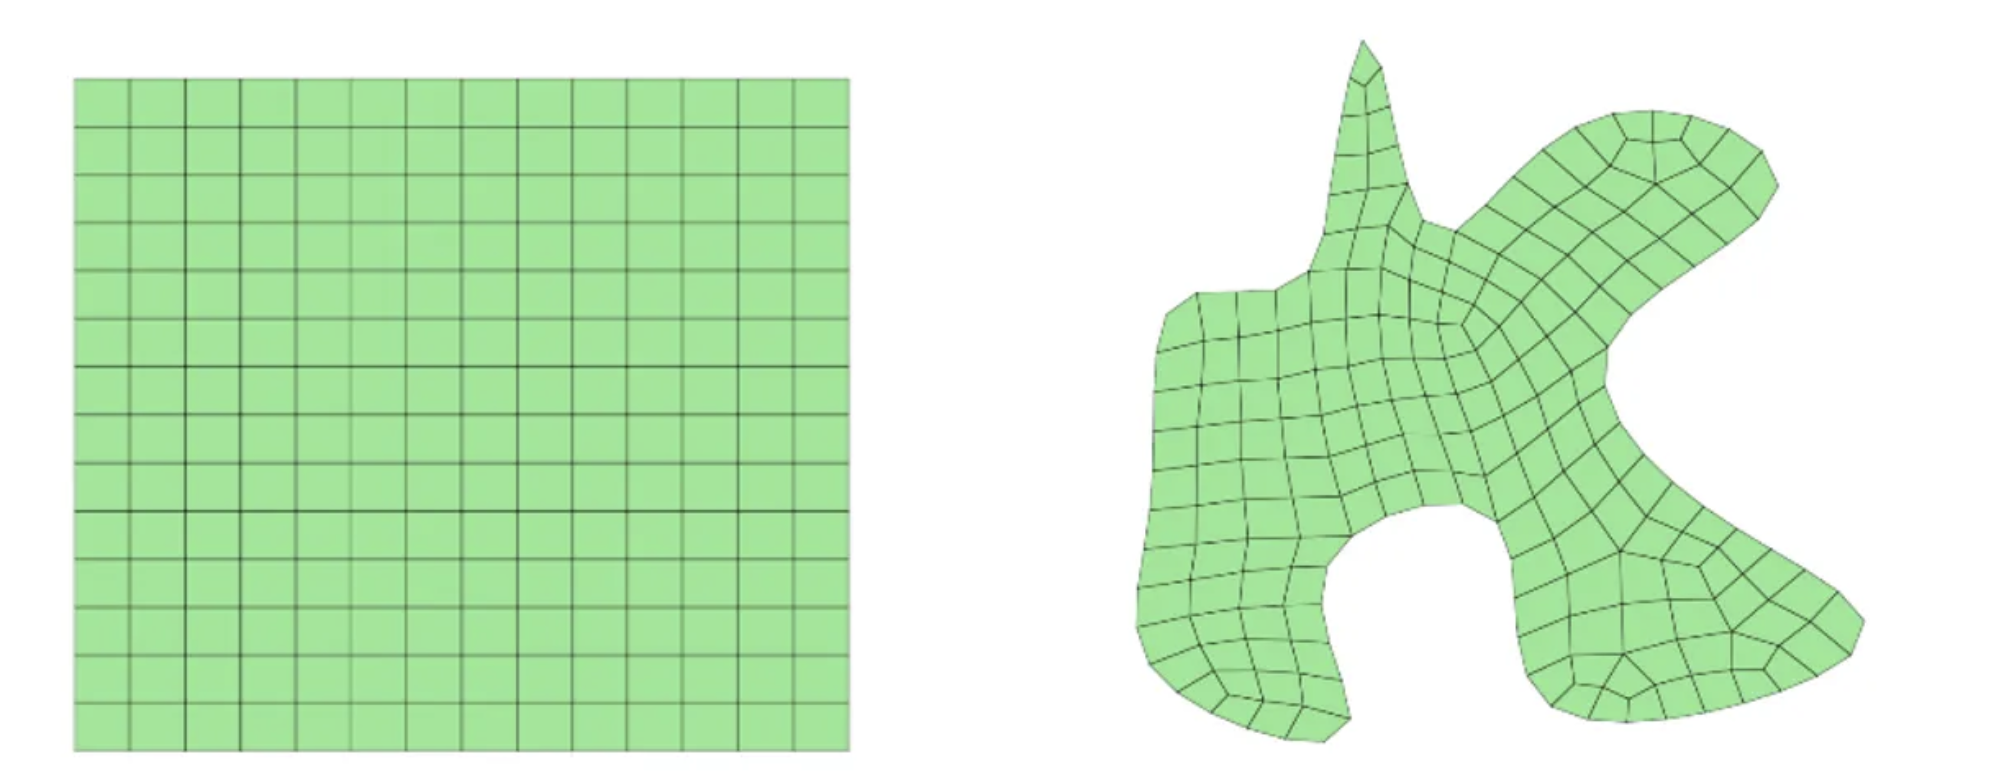
\includegraphics[height=2.5cm]{../images/mesh.png}
  \end{center}
  {\footnotesize (Credit: \hyperlink{https://onscale.com/meshing-in-fea-structured-vs-unstructured-meshes/}{Onscale - structured vs unstructured meshes})}
\end{frame}

{\usebackgroundtemplate{
\includegraphics[height=\paperheight]{../images/inception.jpg}}%
\begin{frame}{Local approach of the finite element method}
  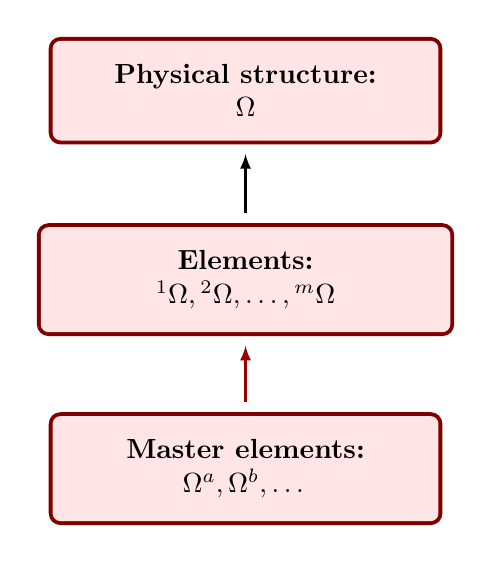
\begin{tikzpicture}[scale=0.8]
    \node (pe) at (-2,6) {
      \begin{tcolorbox}[colframe=red!50!black, colback=red!10, coltitle=black, rounded corners, width=5cm]
        \centering \textbf{Physical structure:} \\ $\Omega$
      \end{tcolorbox}
    };
    \node (ee) at (-2,3) {
      \begin{tcolorbox}[colframe=red!50!black, colback=red!10, coltitle=black, rounded corners,width=5.3cm]
        \centering \textbf{Elements:} \\ ${}^1\Omega,{}^2\Omega,\dots, {}^m\Omega$
      \end{tcolorbox}
    };
    \node (me) at (-2,0) {
      \begin{tcolorbox}[colframe=red!50!black, colback=red!10, coltitle=black, rounded corners,width=5cm]
        \centering \textbf{Master elements:} \\ $\Omega^a,\Omega^b,\dots$
      \end{tcolorbox}
    };
    % Drawing arrows
    \draw[latex-, thick] (pe.south) -- (ee.north);
    \draw[latex-, thick, darkred] (ee.south) -- (me.north);
  \end{tikzpicture}
\end{frame}
}


\begin{frame}{Localization}
  \begin{columns}[T]
    \begin{column}{.4\textwidth}
      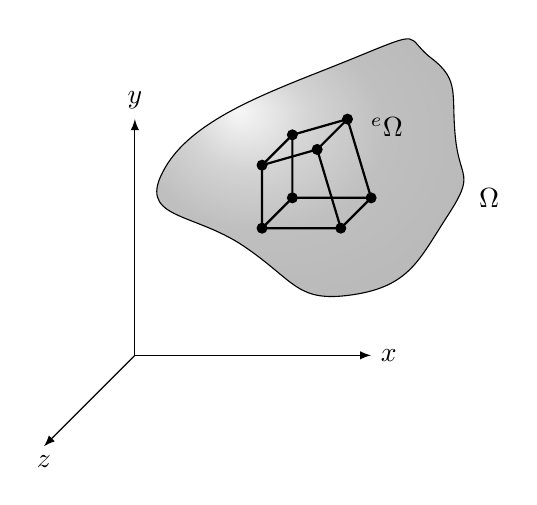
\begin{tikzpicture}
        \draw[-latex] (0,0,0) -- (3,0,0) node[right]{$x$};
        \draw[-latex] (0,0,0) -- (0,3,0) node[above]{$y$};
        \draw[-latex] (0,0,0) -- (0,0,3) node[below]{$z$};
        % Draw the potato-like shape
        \shade [ball color= gray!50!black, opacity=.3] plot [thick,smooth cycle, tension=1] coordinates  {(0,2,-1) (2,3,-2) (3,3,-2) (3.3,2,-2) (3.2,1,-2) (2,0,-2) (1,1,-1)};
        \draw plot [thick,smooth cycle, tension=1] coordinates {(0,2,-1) (2,3,-2) (3,3,-2) (3.3,2,-2) (3.2,1,-2) (2,0,-2) (1,1,-1)};
        % Label the region Omega	
        \node at (3.2,2.9) {${}^e\Omega$};
        % Label the boundary Gamma
        \draw[thick] (2,2,1) -- (2,2.8,1) -- (2.7,3,1) -- (3,2,1) -- cycle;
        \draw[thick] (2,2,0) -- (2,2.8,0) -- (2.7,3,0) -- (3,2,0) -- cycle;
        \draw[thick] (2,2,1) -- (2,2,0);
        \draw[thick] (2,2.8,1) -- (2,2.8,0);
        \draw[thick] (2.7,3,1) -- (2.7,3,0);
        \draw[thick] (3,2,1) -- (3,2,0);
        % Fill vertices
        \foreach \point in {(2,2,1), (2,2.8,1), (2.7,3,1), (3,2,1), (2,2,0), (2,2.8,0), (2.7,3,0), (3,2,0)} {
            \fill \point circle (2pt);
          }
        \node at (4.5,2) {$\Omega$};
      \end{tikzpicture}
    \end{column}
    \hspace{.5cm}
    \begin{column}{.55\textwidth}
      \vspace{.5cm}
      \begin{itemize}
        \setlength\itemsep{1em}
        \item Let $p$ be the number of nodes.
        \item Let $m$ be the number of finite elements in the mesh.
        \item Let ${}^e\Omega$ a generic finite element.
        \item Let ${}^ep$ the number of nodes in the generic element ${}^e\Omega$.
      \end{itemize}
    \end{column}
  \end{columns}
\end{frame}




\begin{frame}{The local finite element point of view (in 2d)}
  \vspace{-1cm}
  \begin{columns}[T]
    \begin{column}{.4\textwidth}
      \begin{center}
        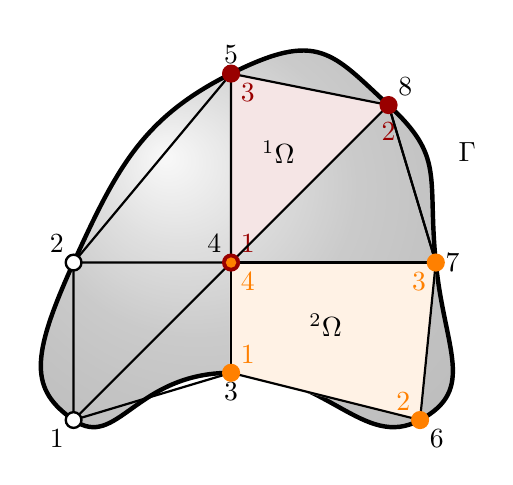
\begin{tikzpicture}[scale=2]
          % \draw[step=1.0,black,thin] (0,0) grid (4,4);
          % Draw the potato-like shape
          \shade [ball color= gray!90!black, opacity=.3] plot [thick,smooth cycle, tension=1] coordinates  {(1,2) (2,3.2) (3,3) (3.3,2) (3.2,1) (2,1.3) (1,1)};
          \draw[ultra thick] plot [thick,smooth cycle, tension=1] coordinates {(1,2) (2,3.2) (3,3) (3.3,2) (3.2,1) (2,1.3) (1,1)};
          \draw[fill=darkred!30,thick,darkred!10] (2,2) -- (3,3) -- (2,3.2) -- cycle;
          \draw[fill=orange!30,thick,orange!10] (2,2) -- (3.3,2) -- (3.2,1) -- (2,1.3) -- cycle;
          % label the nodes
          \node[below left] at (1,1) {$1$};
          \node[above left] at (1,2) {$2$};
          \node[below] at (2,1.3) {$3$};
          \node[orange,above right] at (2,1.3) {$1$};
          \node[above left] at (2,2) {$4$};
          \node[darkred,above right] at (2,2) {$1$};
          \node[orange,below right] at (2,2) {$4$};
          \node[above] at (2,3.2) {$5$};
          \node[darkred,below right] at (2,3.2) {$3$};
          \node[below right] at (3.2,1) {$6$};
          \node[orange,above left] at (3.2,1) {$2$};
          \node[right] at (3.3,2) {$7$};
          \node[orange,below left] at (3.3,2) {$3$};
          \node[above right] at (3,3) {$8$};
          \node[darkred,below={3pt}] at (3,3) {$2$};
          % Label the region Omega
          \node at (2.3,2.7) {${}^1\Omega$};
          \node at (2.6,1.6) {${}^2\Omega$};
          % Label the boundary Gamma
          \node at (3.5,2.7) {$\Gamma$};
          \draw[thick] (1,2) -- (2,3.2) -- (3,3) -- (3.3,2) -- (3.2,1) -- (2,1.3) -- (1,1) -- cycle;
          \draw[thick] (1,2) -- (2,2) -- (3,3) -- (3.3,2);
          \draw[thick] (2,1.3) -- (2,2) -- (3.3,2);
          \draw[thick] (1,1) -- (2,2) -- (2,2.3) -- (2,3.2);
          \node[darkred,draw,shape=circle,fill=darkred,minimum size=2mm,line width=0.3mm,inner sep=0] at (2,2) {};
          \node[orange,draw,shape=circle,fill=orange,minimum size=1mm,line width=0.3mm,inner sep=0] at (2,2) {};
          \node[draw,shape=circle,fill=white,minimum size=2mm,line width=0.3mm,inner sep=0] at (1,1) {};
          \node[draw,shape=circle,fill=white,minimum size=2mm,line width=0.3mm,inner sep=0] at (1,2) {};
          \node[orange,draw,shape=circle,fill=orange,minimum size=2mm,line width=0.3mm,inner sep=0] at (2,1.3) {};
          \node[darkred,draw,shape=circle,fill=darkred,minimum size=2mm,line width=0.3mm,inner sep=0] at (2,3.2) {};
          \node[darkred,draw,shape=circle,fill=darkred,minimum size=2mm,line width=0.3mm,inner sep=0] at (3,3) {};
          \node[orange,draw,shape=circle,fill=orange,minimum size=2mm,line width=0.3mm,inner sep=0] at (3.2,1) {};
          \node[orange,draw,shape=circle,fill=orange,minimum size=2mm,line width=0.3mm,inner sep=0] at (3.3,2) {};
        \end{tikzpicture}
      \end{center}
    \end{column}
    \begin{column}{.6\textwidth}
      Every finite element ${}^e\Omega$ has:
      \begin{itemize}
        \item Number of nodes ${}^ep$,
        \item Connectivity $({}^ep\times 1)$,\vspace{5pt}
        \item ${}^e\mathbf{q}$ vector of nodal displacements ($2{}^e p\times 1$),
        \item ${}^e\mathbf{u}$ vector of displacements ($2\times 1$), \vspace{5pt}
        \item ${}^eh_i$ local shape functions  ($i=1,\dots, {}^ep$),
        \item $^e\mathbf{H}$ local shape functions matrix ($2\times 2{}^e p$), \vspace{5pt}
        \item $^e\mathbf{K}$ local stiffness matrix ($2{}^e p\times 2{}^e p$),
        \item $^e\mathbf{M}$ local mass matrices ($2{}^e p\times2{}^e p$),
        \item $^e\mathbf{r}$ local loads vector ($2{}^e p\times 1$).
      \end{itemize}
    \end{column}
  \end{columns}
\end{frame}

\begin{frame}{Paradigm shift: many with few}
  \vspace{-0.4cm}
  \begin{columns}
    \begin{column}{0.6\textwidth}
      \begin{center}
        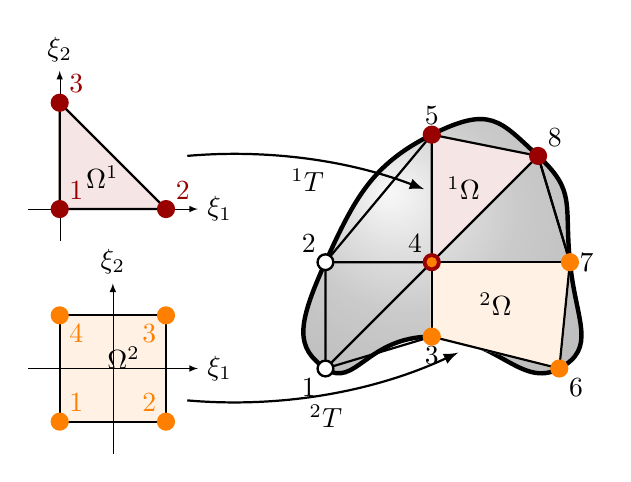
\begin{tikzpicture}[scale=1.35]
          % \draw[step=1.0,black,thin] (-2,0) grid (4,4);
          % Draw the potato-like shape
          \shade [ball color= gray!90!black, opacity=.3] plot [thick,smooth cycle, tension=1] coordinates  {(1,2) (2,3.2) (3,3) (3.3,2) (3.2,1) (2,1.3) (1,1)};
          \draw[ultra thick] plot [thick,smooth cycle, tension=1] coordinates {(1,2) (2,3.2) (3,3) (3.3,2) (3.2,1) (2,1.3) (1,1)};
          \draw[fill=darkred!30,thick,darkred!10] (2,2) -- (3,3) -- (2,3.2) -- cycle;
          \draw[fill=orange!30,thick,orange!10] (2,2) -- (3.3,2) -- (3.2,1) -- (2,1.3) -- cycle;
          % label the nodes
          \node[below left] at (1,1) {$1$};
          \node[above left] at (1,2) {$2$};
          \node[below] at (2,1.3) {$3$};
          \node[above left] at (2,2) {$4$};
          \node[above] at (2,3.2) {$5$};
          \node[below right] at (3.2,1) {$6$};
          \node[right] at (3.3,2) {$7$};
          \node[above right] at (3,3) {$8$};
          % Label the region Omega
          \node at (2.3,2.7) {${}^1\Omega$};
          \node at (2.6,1.6) {${}^2\Omega$};
          \draw[thick] (1,2) -- (2,3.2) -- (3,3) -- (3.3,2) -- (3.2,1) -- (2,1.3) -- (1,1) -- cycle;
          \draw[thick] (1,2) -- (2,2) -- (3,3) -- (3.3,2);
          \draw[thick] (2,1.3) -- (2,2) -- (3.3,2);
          \draw[thick] (1,1) -- (2,2) -- (2,2.3) -- (2,3.2);
          \node[darkred,draw,shape=circle,fill=darkred,minimum size=2mm,line width=0.3mm,inner sep=0] at (2,2) {};
          \node[orange,draw,shape=circle,fill=orange,minimum size=1mm,line width=0.3mm,inner sep=0] at (2,2) {};
          \node[draw,shape=circle,fill=white,minimum size=2mm,line width=0.3mm,inner sep=0] at (1,1) {};
          \node[draw,shape=circle,fill=white,minimum size=2mm,line width=0.3mm,inner sep=0] at (1,2) {};
          \node[orange,draw,shape=circle,fill=orange,minimum size=2mm,line width=0.3mm,inner sep=0] at (2,1.3) {};
          \node[darkred,draw,shape=circle,fill=darkred,minimum size=2mm,line width=0.3mm,inner sep=0] at (2,3.2) {};
          \node[darkred,draw,shape=circle,fill=darkred,minimum size=2mm,line width=0.3mm,inner sep=0] at (3,3) {};
          \node[orange,draw,shape=circle,fill=orange,minimum size=2mm,line width=0.3mm,inner sep=0] at (3.2,1) {};
          \node[orange,draw,shape=circle,fill=orange,minimum size=2mm,line width=0.3mm,inner sep=0] at (3.3,2) {};
          % Draw master square
          \draw[fill=orange!30,thick,orange!10] (-1.5,0.5) -- (-0.5,0.5) -- (-0.5,1.5) -- (-1.5,1.5) -- cycle;
          \draw[thick] (-1.5,0.5) -- (-0.5,0.5) -- (-0.5,1.5) -- (-1.5,1.5) -- cycle;
          \draw[ultra thin,-latex] (-1.8,1) -- (-0.2,1) node[right]{$\xi_1$};
          \draw[ultra thin,-latex] (-1,0.2) -- (-1,1.8) node[above]{$\xi_2$};
          \node at (-0.9,1.1) {$\Omega^2$};
          \draw[thick,-latex] (-0.3,0.7) arc [start angle=-95, end angle=-65, radius=5] node[midway, below]{${}^2T$};
          \node[orange,draw,shape=circle,fill=orange,minimum size=2mm,line width=0.3mm,inner sep=0] at (-1.5,0.5) {};
          \node[orange,draw,shape=circle,fill=orange,minimum size=2mm,line width=0.3mm,inner sep=0] at (-0.5,0.5) {};
          \node[orange,draw,shape=circle,fill=orange,minimum size=2mm,line width=0.3mm,inner sep=0] at (-0.5,1.5) {};
          \node[orange,draw,shape=circle,fill=orange,minimum size=2mm,line width=0.3mm,inner sep=0] at (-1.5,1.5) {};
          \node[orange,above right] at (-1.5,0.5) {$1$};
          \node[orange,below right] at (-1.5,1.5) {$4$};
          \node[orange,above left] at (-0.5,0.5) {$2$};
          \node[orange,below left] at (-0.5,1.5) {$3$};
          % Draw master triangle
          \draw[fill=darkred!30,thick,darkred!10] (-1.5,2.5) -- (-0.5,2.5) -- (-1.5,3.5) -- cycle;
          \draw[thick] (-1.5,2.5) -- (-0.5,2.5) -- (-1.5,3.5) -- cycle;
          \draw[ultra thin,-latex] (-1.8,2.5) -- (-0.2,2.5) node[right]{$\xi_1$};
          \draw[ultra thin,-latex] (-1.5,2.2) -- (-1.5,3.8) node[above]{$\xi_2$};
          \node[darkred,draw,shape=circle,fill=darkred,minimum size=2mm,line width=0.3mm,inner sep=0] at (-1.5,2.5) {};
          \node[darkred,draw,shape=circle,fill=darkred,minimum size=2mm,line width=0.3mm,inner sep=0] at (-0.5,2.5) {};
          \node[darkred,draw,shape=circle,fill=darkred,minimum size=2mm,line width=0.3mm,inner sep=0] at (-1.5,3.5) {};
          \node[darkred,above right] at (-1.5,2.5) {$1$};
          \node[darkred,above right] at (-0.5,2.5) {$2$};
          \node[darkred,above right] at (-1.5,3.5) {$3$};
          \node at (-1.1,2.8) {$\Omega^1$};
          \draw[thick,-latex] (-0.3,3) arc [start angle=95, end angle=69, radius=5] node[midway, below]{${}^1T$};
        \end{tikzpicture}
      \end{center}
    \end{column}
    \begin{column}{0.35\textwidth}
      \begin{itemize}
        \item[\HandRight] {\color{darkred}\textbf{Main idea:}} Local shape functions ${}^eh_i$ are deduced from a \textbf{small set of archetypal shape functions}  ${}^ah_i$ defined on an archetypal element.
      \end{itemize}
    \end{column}
  \end{columns}
  \begin{itemize}
    \item[\HandRight] {\color{darkred}\textbf{Clever idea:}} the transformation ${}^eT$ itself is defined in terms of archetypal shape functions and nodes coordinates:
          \vspace{-0.3cm}
          \[
            {\color{darkred}{}^eT : \mathbf x(\boldxi) = {}^a\mathbf H(\boldxi) ^e{} \mathbf x=\sum_{i=1}^{{}^ep}{}^a h_i(\boldxi){}^e\mathbf x_i       }
          \]
  \end{itemize}
\end{frame}


\begin{frame}{Concrete example: bilinear triangular element (2d)}
  \begin{columns}[T]
    \begin{column}{.45\textwidth}
      \begin{tabular}{c|c|c|c}
        Node  id & Local                        & Node id & Global      \\
        local    & Coord                        & global  & coord.      \\\hline
        1        & \textcolor{darkred}{$(0,0)$} & $4$     & $(x_4,y_4)$ \\
        2        & \textcolor{darkred}{$(1,0)$} & $8$     & $(x_8,y_8)$ \\
        3        & \textcolor{darkred}{$(0,1)$} & $5$     & $(x_5,y_5)$ \\
      \end{tabular}
      \vspace{0.2cm}
      \newline \textbf{Base (archetypal) functions:}
      \vspace{-0.2cm}\begin{align*}
        {}^ah_1 & = 1-\xi_1-\xi_2 \\
        {}^ah_2 & = \xi_1         \\
        {}^ah_3 & = \xi_2
      \end{align*}
    \end{column}
    \begin{column}{.55\textwidth}
      \vspace{0.5cm}
      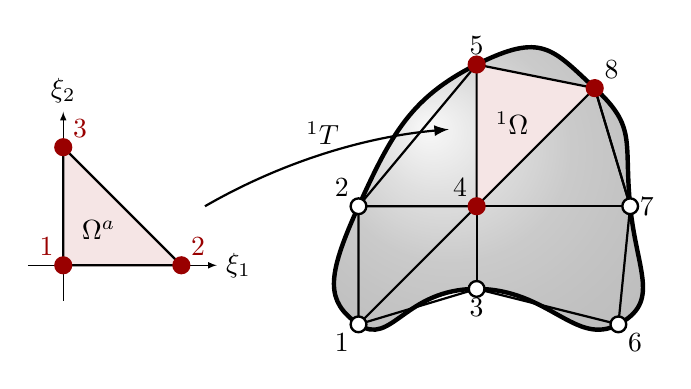
\begin{tikzpicture}[scale=1.5]
        %\draw[step=1.0,black,thin] (-2,0) grid (4,4);
        % Draw the potato-like shape
        \shade [ball color= gray!90!black, opacity=.3] plot [thick,smooth cycle, tension=1] coordinates  {(1,2) (2,3.2) (3,3) (3.3,2) (3.2,1) (2,1.3) (1,1)};
        \draw[ultra thick] plot [thick,smooth cycle, tension=1] coordinates {(1,2) (2,3.2) (3,3) (3.3,2) (3.2,1) (2,1.3) (1,1)};
        \draw[fill=darkred!30,thick,darkred!10] (2,2) -- (3,3) -- (2,3.2) -- cycle;
        % label the nodes
        \node[below left] at (1,1) {$1$};
        \node[above left] at (1,2) {$2$};
        \node[below] at (2,1.3) {$3$};
        \node[above left] at (2,2) {$4$};
        \node[above] at (2,3.2) {$5$};
        \node[below right] at (3.2,1) {$6$};
        \node[right] at (3.3,2) {$7$};
        \node[above right] at (3,3) {$8$};
        % Label the region Omega
        \node at (2.3,2.7) {${}^1\Omega$};
        \draw[thick] (1,2) -- (2,3.2) -- (3,3) -- (3.3,2) -- (3.2,1) -- (2,1.3) -- (1,1) -- cycle;
        \draw[thick] (1,2) -- (2,2) -- (3,3) -- (3.3,2);
        \draw[thick] (2,1.3) -- (2,2) -- (3.3,2);
        \draw[thick] (1,1) -- (2,2) -- (2,2.3) -- (2,3.2);
        \node[darkred,draw,shape=circle,fill=darkred,minimum size=2mm,line width=0.3mm,inner sep=0] at (2,2) {};
        \node[draw,shape=circle,fill=white,minimum size=2mm,line width=0.3mm,inner sep=0] at (1,1) {};
        \node[draw,shape=circle,fill=white,minimum size=2mm,line width=0.3mm,inner sep=0] at (1,2) {};
        \node[draw,shape=circle,fill=white,minimum size=2mm,line width=0.3mm,inner sep=0] at (2,1.3) {};
        \node[darkred,draw,shape=circle,fill=darkred,minimum size=2mm,line width=0.3mm,inner sep=0] at (2,3.2) {};
        \node[darkred,draw,shape=circle,fill=darkred,minimum size=2mm,line width=0.3mm,inner sep=0] at (3,3) {};
        \node[draw,shape=circle,fill=white,minimum size=2mm,line width=0.3mm,inner sep=0] at (3.2,1) {};
        \node[draw,shape=circle,fill=white,minimum size=2mm,line width=0.3mm,inner sep=0] at (3.3,2) {};
        % Draw master triangle
        \draw[fill=darkred!30,thick,darkred!10] (-1.5,1.5) -- (-0.5,1.5) -- (-1.5,2.5) -- cycle;
        \draw[thick] (-1.5,1.5) -- (-0.5,1.5) -- (-1.5,2.5) -- cycle;
        \draw[ultra thin,-latex] (-1.8,1.5) -- (-0.2,1.5) node[right]{$\xi_1$};
        \draw[ultra thin,-latex] (-1.5,1.2) -- (-1.5,2.8) node[above]{$\xi_2$};
        \node[darkred,draw,shape=circle,fill=darkred,minimum size=2mm,line width=0.3mm,inner sep=0] at (-1.5,1.5) {};
        \node[darkred,draw,shape=circle,fill=darkred,minimum size=2mm,line width=0.3mm,inner sep=0] at (-0.5,1.5) {};
        \node[darkred,draw,shape=circle,fill=darkred,minimum size=2mm,line width=0.3mm,inner sep=0] at (-1.5,2.5) {};
        \node[darkred,above left] at (-1.5,1.5) {$1$};
        \node[darkred,above right] at (-0.5,1.5) {$2$};
        \node[darkred,above right] at (-1.5,2.5) {$3$};
        \node at (-1.2,1.8) {$\Omega^a$};
        \draw[thick,-latex] (-0.3,2) arc [start angle=120, end angle=95, radius=5] node[midway, above]{${}^1T$};
      \end{tikzpicture}
    \end{column}
  \end{columns}
  \vspace{0.2cm}
  \hspace{-0.3cm}\textbf{Transformation:}
  $${}^1T:\begin{cases*}
      x(\xi_1,\xi_2) =  x_4 h_1 + x_8 h_2 + x_5 h_3  = x_4+(x_8-x_4)\xi_1+(x_5-x_4)\xi_2 \\
      y(\xi_1,\xi_2)=  y_4 h_1 + y_8 h_2 + y_5 h_3 = y_4+(y_8-y_4)\xi_1+(y_5-y_4)\xi_2
    \end{cases*}$$
\end{frame}


\begin{frame}{Consequence: integration over archetypal elements}
  \begin{align*}
    \int_{{\color{darkred}{}^e\Omega}}(\dots)d\Omega & \quad{\color{darkred}\xmapsto[]{\text{replaced by}}}\quad\int_{{\color{darkred}\Omega{}^a}}(\dots)\, {}^ej d\xi_1d\xi_2                                         \\[5pt]
    \frac{\partial}{\partial x_i}                    & \quad{\color{darkred}\xmapsto[]{\text{replaced by}}}\quad\frac{\partial\xi_1}{\partial x_i}\partial_{\xi_1}+ \frac{\partial\xi_2}{\partial x_i}\partial_{\xi_2}
  \end{align*}
  where ${}^ej$ is the determinant of the Jacobian matrix ${}^e\mathbf J$ of the transformation ${}^eT$.
  \vspace{0.2cm}
  \begin{tcolorbox}[colback=darkred!10,colframe=darkred!40!black,]
    \begin{itemize}
      \item[\HandRight] For each transformation, it is necessary to compute the Jacobian matrix, its determinant, and its inverse.
    \end{itemize}
  \end{tcolorbox}
\end{frame}

\begin{frame}{Concrete example: local mass and stiffness matrices}
  \begin{itemize}
    \item\textbf{Local mass matrix:}
          \begin{align*}
            {}^1\mathbf M & =\int_{\Omega^a} \rho\, {}^a\mathbf H^T{}^a\mathbf H \, {}^1j \, d\boldxi                                 \\
                          & = \int_{\Omega^a} \rho\begin{bmatrix}
                                                    {}^a h_1^2 \mathbf I      & {}^a h_1{}^a h_2 \mathbf I & {}^a h_1{}^a h_3 \mathbf I \\
                                                    {}^ah_2{}^a h_1 \mathbf I & {}^a h_2^2 \mathbf I       & {}^a h_2{}^a h_3 \mathbf I \\
                                                    {}^ah_3{}^a h_1 \mathbf I & {}^a h_3{}^a h_2 \mathbf I & {}^a h_3^2 \mathbf I       \\
                                                  \end{bmatrix} \, {}^1j \, d\xi_2d\xi_1
          \end{align*}

    \item \textbf{Local stiffness matrix:}
          $$
            {}^1\mathbf K = \int_{\Omega^a} \begin{bmatrix}
              \dots &                                                                                                                            & \dots \\
                    & \left(\nabla_{\boldxi}{}^ah_i {}^1\mathbf J^{-1}\right)^T\mathbf C\left( \nabla_{\boldxi}{}^ah_j {}^1\mathbf J^{-1}\right) &       \\
              \dots &                                                                                                                            & \dots \\
            \end{bmatrix} \, {}^1j \, d\xi_2d\xi_1
          $$
  \end{itemize}
\end{frame}

\begin{frame}{Assembly of the mass matrix: local to global}
  \vspace{-0.7cm}
  $$
    {}^1\mathbf M
    = \int_{\Omega^a} \rho\begin{bmatrix}
      {}^a h_1^2 \mathbf I      & {}^a h_1{}^a h_2 \mathbf I & {}^a h_1{}^a h_3 \mathbf I \\
      {}^ah_2{}^a h_1 \mathbf I & {}^a h_2^2 \mathbf I       & {}^a h_2{}^a h_3 \mathbf I \\
      {}^ah_3{}^a h_1 \mathbf I & {}^a h_3{}^a h_2 \mathbf I & {}^a h_3^2 \mathbf I       \\
    \end{bmatrix} \, {}^ej \, d\xi_2d\xi_1=\begin{bmatrix}
      {}^1\mathbf M_{11} & {}^1\mathbf M_{12} & {}^1\mathbf M_{13} \\
      {}^1\mathbf M_{21} & {}^1\mathbf M_{22} & {}^1\mathbf M_{23} \\
      {}^1\mathbf M_{31} & {}^1\mathbf M_{32} & {}^1\mathbf M_{33} \\
    \end{bmatrix}$$
  We assembly local mass matrices into the global ones using the assembly operator:
  \begin{columns}
    \begin{column}{0.7\textwidth}
      \vspace{0.5cm}
      $$    \mathbf M =\A_{e=1}^m {}^e\mathbf M = \sum_{e=1}^{m} {}^e\mathbf L^T {}^e\mathbf M{}^e\mathbf L$$
      \hspace{0.7cm}where
      $${}^1\mathbf L=\begin{bmatrix}
          \mathbf 0 & \mathbf 0 & \mathbf 0 & \mathbf I & \mathbf 0 & \mathbf 0 & \mathbf 0 & \mathbf 0 & \\
          \mathbf 0 & \mathbf 0 & \mathbf 0 & \mathbf 0 & \mathbf 0 & \mathbf 0 & \mathbf 0 & \mathbf I & \\
          \mathbf 0 & \mathbf 0 & \mathbf 0 & \mathbf 0 & \mathbf I & \mathbf 0 & \mathbf 0 & \mathbf 0 & \\
        \end{bmatrix}$$
    \end{column}
    \hspace{1cm}
    \begin{column}{0.3\textwidth}
      \begin{tabular}{c|c}
        Node  id. & Node  id. \\
        local     & global    \\\hline
        1         & $4$       \\
        2         & $8$       \\
        3         & $5$       \\
      \end{tabular}
    \end{column}
  \end{columns}
\end{frame}

\begin{frame}{Assembly of the mass matrix: local to global}
  $$    {}^1\mathbf L^T {}^1\mathbf M{}^1\mathbf L=\begin{bmatrix}
      \mathbf 0 & \mathbf 0 & \mathbf 0 & \mathbf 0          & \mathbf 0          & \mathbf 0 & \mathbf 0 & \mathbf 0          & \\
      \mathbf 0 & \mathbf 0 & \mathbf 0 & \mathbf 0          & \mathbf 0          & \mathbf 0 & \mathbf 0 & \mathbf 0          & \\
      \mathbf 0 & \mathbf 0 & \mathbf 0 & \mathbf 0          & \mathbf 0          & \mathbf 0 & \mathbf 0 & \mathbf 0          & \\
      \mathbf 0 & \mathbf 0 & \mathbf 0 & {}^1\mathbf M_{11} & {}^1\mathbf M_{13} & \mathbf 0 & \mathbf 0 & {}^1\mathbf M_{12} & \\
      \mathbf 0 & \mathbf 0 & \mathbf 0 & {}^1\mathbf M_{31} & {}^1\mathbf M_{33} & \mathbf 0 & \mathbf 0 & {}^1\mathbf M_{32} & \\
      \mathbf 0 & \mathbf 0 & \mathbf 0 & \mathbf 0          & \mathbf 0          & \mathbf 0 & \mathbf 0 & \mathbf 0          & \\
      \mathbf 0 & \mathbf 0 & \mathbf 0 & \mathbf 0          & \mathbf 0          & \mathbf 0 & \mathbf 0 & \mathbf 0          & \\
      \mathbf 0 & \mathbf 0 & \mathbf 0 & {}^1\mathbf M_{21} & {}^1\mathbf M_{23} & \mathbf 0 & \mathbf 0 & {}^1\mathbf M_{22} & \\
    \end{bmatrix}$$
\end{frame}

\begin{frame}{Three-dimensional families of finite elements}
  \begin{center}
    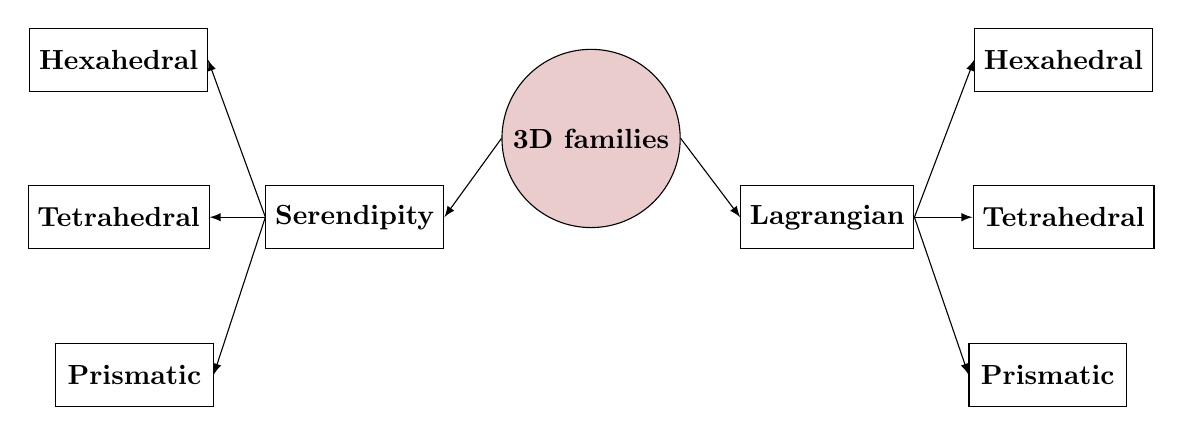
\begin{tikzpicture}
      % Draw the main circle labeled "3D"
      \node[circle, draw, minimum size=1cm, fill=darkred!20] (circle) at (0,1) {\textbf{3D families}};
      % Draw rectangles first column
      \node[draw, minimum width=2cm, minimum height=0.8cm] (hex) at (6,2) {\textbf{Hexahedral}};
      \node[draw, minimum width=2cm, minimum height=0.8cm] (tet) at (6,0) {\textbf{Tetrahedral}};
      \node[draw, minimum width=2cm, minimum height=0.8cm] (pri) at (5.8,-2) {\textbf{Prismatic}};
      \node[draw, minimum width=2cm, minimum height=0.8cm] (lag) at (3,0){\textbf{Lagrangian}};
      \node[draw, minimum width=2cm, minimum height=0.8cm] (ser) at (-3,0){\textbf{Serendipity}};
      \node[draw, minimum width=2cm, minimum height=0.8cm] (hexSer) at (-6,2) {\textbf{Hexahedral}};
      \node[draw, minimum width=2cm, minimum height=0.8cm] (tetSer) at (-6,0) {\textbf{Tetrahedral}};
      \node[draw, minimum width=2cm, minimum height=0.8cm] (priSer) at (-5.8,-2) {\textbf{Prismatic}};
      % Draw connecting arrows
      \draw[-latex] (circle.east) -- (lag.west);
      \draw[-latex] (circle.west) -- (ser.east);
      \draw[-latex] (lag.east) -- (hex.west);
      \draw[-latex] (lag.east) -- (tet.west);
      \draw[-latex] (lag.east) -- (pri.west);
      \draw[-latex] (ser.west) -- (hexSer.east);
      \draw[-latex] (ser.west) -- (tetSer.east);
      \draw[-latex] (ser.west) -- (priSer.east);
    \end{tikzpicture}
  \end{center}
\end{frame}

\begin{frame}{Hexahedral elements}
  \begin{columns}
    \begin{column}{0.33\textwidth}
      \centering
      \textbf{Trilinear \\ Lagrangian}
      \vspace{0.4cm}

      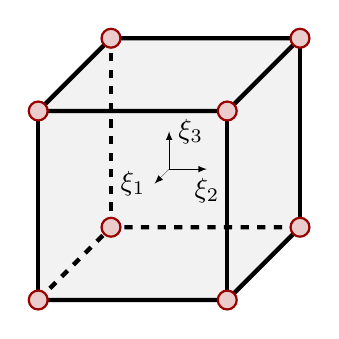
\begin{tikzpicture}[scale=1.2]
        \def\a{1}
        \coordinate (x1) at (-\a, -\a,-\a);
        \coordinate (x4) at (\a, -\a,-\a);
        \coordinate (x8) at (\a, \a,-\a);
        \coordinate (x5) at (-\a, \a,-\a);
        \coordinate (x2) at (-\a, -\a,\a);
        \coordinate (x3) at (\a, -\a,\a);
        \coordinate (x7) at (\a, \a,\a);
        \coordinate (x6) at (-\a, \a,\a);
        %Shade
        \filldraw[gray!10] (x1) -- (x2) -- (x3) -- (x4) -- cycle;
        \filldraw[gray!10] (x2) -- (x3) -- (x7) -- (x6) -- cycle;
        \filldraw[gray!10] (x3) -- (x4) -- (x8) -- (x7) -- cycle;
        \filldraw[gray!10] (x6) -- (x7) -- (x8) -- (x5) -- cycle;
        %Axis
        %Axis
        \draw[-latex,ultra thin] (0,0,0) -- (0.4,0,0) node[below]{$\xi_2$};
        \draw[-latex,ultra thin] (0,0,0) -- (0,0.4,0) node[right]{$\xi_3$};
        \draw[-latex,ultra thin] (0,0,0) -- (0,0,0.4) node[left]{$\xi_1$};
        %Draw edges
        \draw[ultra thick] (x6) -- (x7) -- (x8) -- (x5) -- cycle;
        \draw[ultra thick] (x2) -- (x3) -- (x4);
        \draw[ultra thick,dashed] (x2) -- (x1) -- (x4);
        \draw[ultra thick] (x2) -- (x6);
        \draw[ultra thick] (x3) -- (x7);
        \draw[ultra thick] (x4) -- (x8);
        \draw[ultra thick,dashed] (x1) -- (x5);
        %Draw nodes
        \draw[fill=darkred!20, thick,draw=darkred] (x1)  circle(0.1cm);
        \draw[fill=darkred!20, thick,draw=darkred] (x2)  circle(0.1cm);
        \draw[fill=darkred!20, thick,draw=darkred] (x3)  circle(0.1cm);
        \draw[fill=darkred!20, thick,draw=darkred] (x4)  circle(0.1cm);
        \draw[fill=darkred!20, thick,draw=darkred] (x5)  circle(0.1cm);
        \draw[fill=darkred!20, thick,draw=darkred] (x6)  circle(0.1cm);
        \draw[fill=darkred!20, thick,draw=darkred] (x7)  circle(0.1cm);
        \draw[fill=darkred!20, thick,draw=darkred] (x8)  circle(0.1cm);
      \end{tikzpicture}
    \end{column}
    \begin{column}{0.33\textwidth}
      \centering
      \textbf{Triquadratic Lagrangian}
      \vspace{0.4cm}

      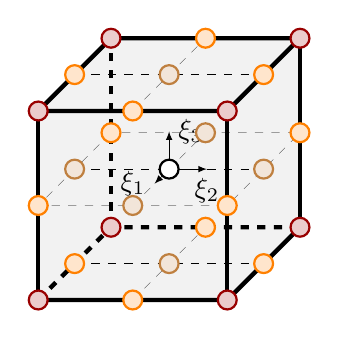
\begin{tikzpicture}[scale=1.2]
        \def\a{1}
        \coordinate (x1) at (-\a, -\a,-\a);
        \coordinate (x9) at (-\a, -\a,0);
        \coordinate (x2) at (-\a, -\a,\a);
        \coordinate (x10) at (0, -\a,\a);
        \coordinate (x3) at (\a, -\a,\a);
        \coordinate (x11) at (\a, -\a,0);
        \coordinate (x4) at (\a, -\a,-\a);
        \coordinate (x12) at (0, -\a,-\a);
        \coordinate (x5) at (-\a, \a,-\a);
        \coordinate (x13) at (-\a, \a,0);
        \coordinate (x6) at (-\a, \a,\a);
        \coordinate (x14) at (0, \a,\a);
        \coordinate (x7) at (\a, \a,\a);
        \coordinate (x15) at (\a, \a,0);
        \coordinate (x8) at (\a, \a,-\a);
        \coordinate (x16) at (0, \a,-\a);
        \coordinate (x17) at (-\a, 0,-\a);
        \coordinate (x18) at (-\a, 0,\a);
        \coordinate (x19) at (\a, 0,\a);
        \coordinate (x20) at (\a, 0,-\a);
        \coordinate (x21) at (0, -\a,0);
        \coordinate (x22) at (0, \a,0);
        \coordinate (x23) at (-\a, 0,0);
        \coordinate (x24) at (0, 0,\a);
        \coordinate (x25) at (\a, 0,0);
        \coordinate (x26) at (0, 0,-\a);
        \coordinate (x27) at (0,0,0);
        %Shade
        \filldraw[gray!10] (x1) -- (x2) -- (x3) -- (x4) -- cycle;
        \filldraw[gray!10] (x2) -- (x3) -- (x7) -- (x6) -- cycle;
        \filldraw[gray!10] (x3) -- (x4) -- (x8) -- (x7) -- cycle;
        \filldraw[gray!10] (x6) -- (x7) -- (x8) -- (x5) -- cycle;
        %Axis
        \draw[-latex,ultra thin] (0,0,0) -- (0.4,0,0) node[below]{$\xi_2$};
        \draw[-latex,ultra thin] (0,0,0) -- (0,0.4,0) node[right]{$\xi_3$};
        \draw[-latex,ultra thin] (0,0,0) -- (0,0,0.4) node[left]{$\xi_1$};
        %Draw edges
        \draw[ultra thick] (x6) -- (x7) -- (x8) -- (x5) -- cycle;
        \draw[ultra thick] (x2) -- (x3) -- (x4);
        \draw[ultra thick,dashed] (x2) -- (x1) -- (x4);
        \draw[ultra thick] (x2) -- (x6);
        \draw[ultra thick] (x3) -- (x7);
        \draw[ultra thick] (x4) -- (x8);
        \draw[ultra thick,dashed] (x1) -- (x5);
        \draw[ultra thin,dashed] (x17) -- (x18) -- (x19) -- (x20) -- (x17);
        \draw[ultra thin,dashed] (x23) -- (x25);
        \draw[ultra thin,dashed] (x24) -- (x26);
        \draw[ultra thin,dashed] (x9) -- (x11);
        \draw[ultra thin,dashed] (x10) -- (x12);
        \draw[ultra thin,dashed] (x13) -- (x15);
        \draw[ultra thin,dashed] (x14) -- (x16);
        %Draw nodes
        \draw[fill=darkred!20, thick,draw=darkred] (x1) circle(0.1cm);
        \draw[fill=darkred!20, thick,draw=darkred] (x2) circle(0.1cm);
        \draw[fill=darkred!20, thick,draw=darkred] (x3) circle(0.1cm);
        \draw[fill=darkred!20, thick,draw=darkred] (x4) circle(0.1cm);
        \draw[fill=darkred!20, thick,draw=darkred] (x5) circle(0.1cm);
        \draw[fill=darkred!20, thick,draw=darkred] (x6) circle(0.1cm);
        \draw[fill=darkred!20, thick,draw=darkred] (x7) circle(0.1cm);
        \draw[fill=darkred!20, thick,draw=darkred] (x8) circle(0.1cm);
        \draw[fill=orange!20, thick,draw=orange] (x9) circle(0.1cm);
        \draw[fill=orange!20, thick,draw=orange] (x10) circle(0.1cm);
        \draw[fill=orange!20, thick,draw=orange] (x11) circle(0.1cm);
        \draw[fill=orange!20, thick,draw=orange] (x12) circle(0.1cm);
        \draw[fill=orange!20, thick,draw=orange] (x13) circle(0.1cm);
        \draw[fill=orange!20, thick,draw=orange] (x14) circle(0.1cm);
        \draw[fill=orange!20, thick,draw=orange] (x15) circle(0.1cm);
        \draw[fill=orange!20, thick,draw=orange] (x16) circle(0.1cm);
        \draw[fill=orange!20, thick,draw=orange] (x17) circle(0.1cm);
        \draw[fill=orange!20, thick,draw=orange] (x18) circle(0.1cm);
        \draw[fill=orange!20, thick,draw=orange] (x19) circle(0.1cm);
        \draw[fill=orange!20, thick,draw=orange] (x20) circle(0.1cm);
        \draw[fill=brown!20, thick,draw=brown] (x21) circle(0.1cm);
        \draw[fill=brown!20, thick,draw=brown] (x22) circle(0.1cm);
        \draw[fill=brown!20, thick,draw=brown] (x23) circle(0.1cm);
        \draw[fill=brown!20, thick,draw=brown] (x24) circle(0.1cm);
        \draw[fill=brown!20, thick,draw=brown] (x25) circle(0.1cm);
        \draw[fill=brown!20, thick,draw=brown] (x26) circle(0.1cm);
        \draw[fill=white, thick] (x27) circle(0.1cm);
      \end{tikzpicture}
    \end{column}
    \begin{column}{0.33\textwidth}
      \centering
      \textbf{Triquadratic serendipity}
      \vspace{0.4cm}

      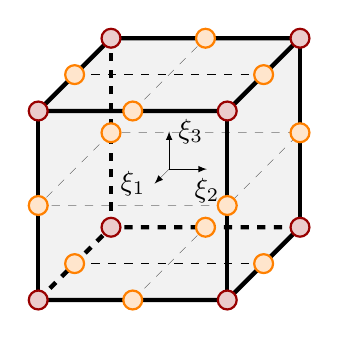
\begin{tikzpicture}[scale=1.2]
        \def\a{1}
        \coordinate (x1) at (-\a, -\a,-\a);
        \coordinate (x9) at (-\a, -\a,0);
        \coordinate (x2) at (-\a, -\a,\a);
        \coordinate (x10) at (0, -\a,\a);
        \coordinate (x3) at (\a, -\a,\a);
        \coordinate (x11) at (\a, -\a,0);
        \coordinate (x4) at (\a, -\a,-\a);
        \coordinate (x12) at (0, -\a,-\a);
        \coordinate (x5) at (-\a, \a,-\a);
        \coordinate (x13) at (-\a, \a,0);
        \coordinate (x6) at (-\a, \a,\a);
        \coordinate (x14) at (0, \a,\a);
        \coordinate (x7) at (\a, \a,\a);
        \coordinate (x15) at (\a, \a,0);
        \coordinate (x8) at (\a, \a,-\a);
        \coordinate (x16) at (0, \a,-\a);
        \coordinate (x17) at (-\a, 0,-\a);
        \coordinate (x18) at (-\a, 0,\a);
        \coordinate (x19) at (\a, 0,\a);
        \coordinate (x20) at (\a, 0,-\a);
        %Shade
        \filldraw[gray!10] (x1) -- (x2) -- (x3) -- (x4) -- cycle;
        \filldraw[gray!10] (x2) -- (x3) -- (x7) -- (x6) -- cycle;
        \filldraw[gray!10] (x3) -- (x4) -- (x8) -- (x7) -- cycle;
        \filldraw[gray!10] (x6) -- (x7) -- (x8) -- (x5) -- cycle;
        %Axis
        \draw[-latex,ultra thin] (0,0,0) -- (0.4,0,0) node[below]{$\xi_2$};
        \draw[-latex,ultra thin] (0,0,0) -- (0,0.4,0) node[right]{$\xi_3$};
        \draw[-latex,ultra thin] (0,0,0) -- (0,0,0.4) node[left]{$\xi_1$};
        %Draw edges
        \draw[ultra thick] (x6) -- (x7) -- (x8) -- (x5) -- cycle;
        \draw[ultra thick] (x2) -- (x3) -- (x4);
        \draw[ultra thick,dashed] (x2) -- (x1) -- (x4);
        \draw[ultra thick] (x2) -- (x6);
        \draw[ultra thick] (x3) -- (x7);
        \draw[ultra thick] (x4) -- (x8);
        \draw[ultra thick,dashed] (x1) -- (x5);
        \draw[ultra thin,dashed] (x9) -- (x11);
        \draw[ultra thin,dashed] (x10) -- (x12);
        \draw[ultra thin,dashed] (x13) -- (x15);
        \draw[ultra thin,dashed] (x14) -- (x16);
        \draw[ultra thin,dashed] (x17) -- (x18) -- (x19) -- (x20) -- cycle;
        %Draw nodes
        \draw[fill=darkred!20, thick,draw=darkred] (x1) circle(0.1cm);
        \draw[fill=darkred!20, thick,draw=darkred] (x2) circle(0.1cm);
        \draw[fill=darkred!20, thick,draw=darkred] (x3) circle(0.1cm);
        \draw[fill=darkred!20, thick,draw=darkred] (x4) circle(0.1cm);
        \draw[fill=darkred!20, thick,draw=darkred] (x5) circle(0.1cm);
        \draw[fill=darkred!20, thick,draw=darkred] (x6) circle(0.1cm);
        \draw[fill=darkred!20, thick,draw=darkred] (x7) circle(0.1cm);
        \draw[fill=darkred!20, thick,draw=darkred] (x8) circle(0.1cm);
        \draw[fill=orange!20, thick,draw=orange] (x9) circle(0.1cm);
        \draw[fill=orange!20, thick,draw=orange] (x10) circle(0.1cm);
        \draw[fill=orange!20, thick,draw=orange] (x11) circle(0.1cm);
        \draw[fill=orange!20, thick,draw=orange] (x12) circle(0.1cm);
        \draw[fill=orange!20, thick,draw=orange] (x13) circle(0.1cm);
        \draw[fill=orange!20, thick,draw=orange] (x14) circle(0.1cm);
        \draw[fill=orange!20, thick,draw=orange] (x15) circle(0.1cm);
        \draw[fill=orange!20, thick,draw=orange] (x16) circle(0.1cm);
        \draw[fill=orange!20, thick,draw=orange] (x17) circle(0.1cm);
        \draw[fill=orange!20, thick,draw=orange] (x18) circle(0.1cm);
        \draw[fill=orange!20, thick,draw=orange] (x19) circle(0.1cm);
        \draw[fill=orange!20, thick,draw=orange] (x20) circle(0.1cm);
      \end{tikzpicture}
    \end{column}
  \end{columns}
\end{frame}

\begin{frame}{Tetrahedral elements}
  \begin{columns}
    \begin{column}{0.33\textwidth}
      \centering
      \textbf{Trilinear \\ Lagrangian}
      \vspace{0.4cm}

      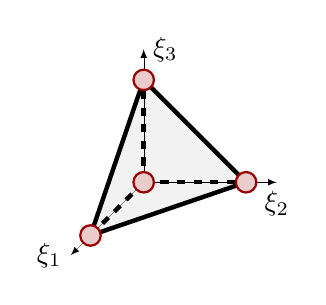
\begin{tikzpicture}[scale=1.3]
        \def\a{1}
        \def\b{1.35}
        \coordinate (x1) at (0,0,0);
        \coordinate (x2) at (0,0,\b);
        \coordinate (x3) at (\a,0,0);
        \coordinate (x4) at (0, \a,0);
        %Shade
        \filldraw[gray!10] (x2) -- (x3) -- (x4) -- cycle;
        %Axis
        \draw[-latex,ultra thin] (0,0,0) -- (\a+0.3,0,0) node[below]{$\xi_2$};
        \draw[-latex,ultra thin] (0,0,0) -- (0,\a+0.3,0) node[right]{$\xi_3$};
        \draw[-latex,ultra thin] (0,0,0) -- (0,0,\b+0.5) node[left]{$\xi_1$};
        %Draw edges
        \draw[ultra thick,dashed] (x1) -- (x4);
        \draw[ultra thick,dashed] (x1) -- (x2);
        \draw[ultra thick,dashed] (x1) -- (x3);
        \draw[ultra thick] (x2) -- (x3) -- (x4) -- cycle;
        %Draw nodes
        \draw[fill=darkred!20, thick,draw=darkred] (x1) circle(0.1cm);
        \draw[fill=darkred!20, thick,draw=darkred] (x2) circle(0.1cm);
        \draw[fill=darkred!20, thick,draw=darkred] (x3) circle(0.1cm);
        \draw[fill=darkred!20, thick,draw=darkred] (x4) circle(0.1cm);
      \end{tikzpicture}
    \end{column}
    \begin{column}{0.33\textwidth}
      \centering
      \textbf{Triquadratic Lagrangian}
      \vspace{0.4cm}

      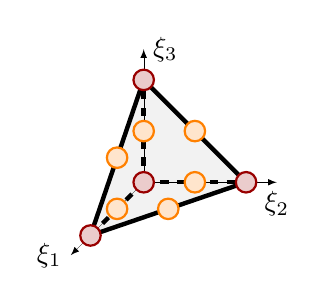
\begin{tikzpicture}[scale=1.3]
        \def\a{1}
        \def\b{1.35}
        \coordinate (x1) at (0,0,0);
        \coordinate (x2) at (0,0,\b);
        \coordinate (x3) at (\a,0,0);
        \coordinate (x4) at (0, \a,0);
        \coordinate (x5) at (0,0,\b/2);
        \coordinate (x6) at (\a/2,0,\b/2);
        \coordinate (x7) at (\a/2,0,0);
        \coordinate (x8) at (0,\a/2,0);
        \coordinate (x9) at (0,\a/2,\b/2);
        \coordinate (x10) at (\a/2,\a/2,0);
        %Shade
        \filldraw[gray!10] (x2) -- (x3) -- (x4) -- cycle;
        %Axis
        \draw[-latex,ultra thin] (0,0,0) -- (\a+0.3,0,0) node[below]{$\xi_2$};
        \draw[-latex,ultra thin] (0,0,0) -- (0,\a+0.3,0) node[right]{$\xi_3$};
        \draw[-latex,ultra thin] (0,0,0) -- (0,0,\b+0.5) node[left]{$\xi_1$};
        %Draw edges
        \draw[ultra thick,dashed] (x1) -- (x4);
        \draw[ultra thick,dashed] (x1) -- (x2);
        \draw[ultra thick,dashed] (x1) -- (x3);
        \draw[ultra thick] (x2) -- (x3) -- (x4) -- cycle;
        %Draw nodes
        \draw[fill=darkred!20, thick,draw=darkred] (x1)  circle(0.1cm);
        \draw[fill=darkred!20, thick,draw=darkred] (x2)  circle(0.1cm);
        \draw[fill=darkred!20, thick,draw=darkred] (x3)  circle(0.1cm);
        \draw[fill=darkred!20, thick,draw=darkred] (x4)  circle(0.1cm);
        \draw[fill=orange!20, thick,draw=orange] (x5)  circle(0.1cm);
        \draw[fill=orange!20, thick,draw=orange] (x6)  circle(0.1cm);
        \draw[fill=orange!20, thick,draw=orange] (x7)  circle(0.1cm);
        \draw[fill=orange!20, thick,draw=orange] (x8)  circle(0.1cm);
        \draw[fill=orange!20, thick,draw=orange] (x9)  circle(0.1cm);
        \draw[fill=orange!20, thick,draw=orange] (x10)  circle(0.1cm);
      \end{tikzpicture}
    \end{column}
    \begin{column}{0.33\textwidth}
      \centering
      \textbf{Triquadratic serendipity}
      \vspace{0.4cm}

      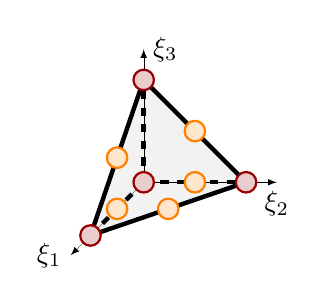
\begin{tikzpicture}[scale=1.3]
        \def\a{1}
        \def\b{1.35}
        \coordinate (x1) at (0,0,0);
        \coordinate (x2) at (0,0,\b);
        \coordinate (x3) at (\a,0,0);
        \coordinate (x4) at (0, \a,0);
        \coordinate (x5) at (0,0,\b/2);
        \coordinate (x6) at (\a/2,0,\b/2);
        \coordinate (x7) at (\a/2,0,0);
        \coordinate (x8) at (0,\a/2,\b/2);
        \coordinate (x9) at (\a/2,\a/2,0);
        %Shade
        \filldraw[gray!10] (x2) -- (x3) -- (x4) -- cycle;
        %Axis
        \draw[-latex,ultra thin] (0,0,0) -- (\a+0.3,0,0) node[below]{$\xi_2$};
        \draw[-latex,ultra thin] (0,0,0) -- (0,\a+0.3,0) node[right]{$\xi_3$};
        \draw[-latex,ultra thin] (0,0,0) -- (0,0,\b+0.5) node[left]{$\xi_1$};
        %Draw edges
        \draw[ultra thick,dashed] (x1) -- (x4);
        \draw[ultra thick,dashed] (x1) -- (x2);
        \draw[ultra thick,dashed] (x1) -- (x3);
        \draw[ultra thick] (x2) -- (x3) -- (x4) -- cycle;
        %Draw nodes
        \draw[fill=darkred!20, thick,draw=darkred] (x1) circle(0.1cm);
        \draw[fill=darkred!20, thick,draw=darkred] (x2)  circle(0.1cm);
        \draw[fill=darkred!20, thick,draw=darkred] (x3)  circle(0.1cm);
        \draw[fill=darkred!20, thick,draw=darkred] (x4)  circle(0.1cm);
        \draw[fill=orange!20, thick,draw=orange] (x5)  circle(0.1cm);
        \draw[fill=orange!20, thick,draw=orange] (x6)  circle(0.1cm);
        \draw[fill=orange!20, thick,draw=orange] (x7)  circle(0.1cm);
        \draw[fill=orange!20, thick,draw=orange] (x8)  circle(0.1cm);
        \draw[fill=orange!20, thick,draw=orange] (x9)  circle(0.1cm);
      \end{tikzpicture}
    \end{column}
  \end{columns}
\end{frame}

\begin{frame}{Prismatic elements}
  \begin{columns}
    \begin{column}{0.33\textwidth}
      \centering
      \textbf{Trilinear \\ Lagrangian}
      \vspace{0.4cm}

      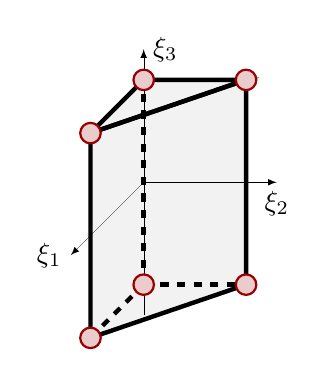
\begin{tikzpicture}[scale=1.3]
        \def\a{1}
        \def\b{1.35}
        \coordinate (x1) at (0,-\a,0);
        \coordinate (x2) at (0,-\a,\b);
        \coordinate (x3) at (\a,-\a,0);
        \coordinate (x4) at (0, \a,0);
        \coordinate (x5) at (0, \a,\b);
        \coordinate (x6) at (\a,\a,0);
        %Shade
        \filldraw[gray!10] (x2) -- (x3) -- (x6) -- (x4) -- (x5) -- (x2);
        %Axis
        \draw[-latex,ultra thin] (0,0,0) -- (\a+0.3,0,0) node[below]{$\xi_2$};
        \draw[-latex,ultra thin] (0,-\a-0.3,0) -- (0,\a+0.3,0) node[right]{$\xi_3$};
        \draw[-latex,ultra thin] (0,0,0) -- (0,0,\b+0.5) node[left]{$\xi_1$};
        %Draw edges
        \draw[ultra thick,dashed] (x1) -- (x4);
        \draw[ultra thick,dashed] (x1) -- (x2);
        \draw[ultra thick,dashed] (x1) -- (x3);
        \draw[ultra thick] (x5) -- (x4) -- (x6) -- cycle;
        \draw[ultra thick] (x6) -- (x3) -- (x2) -- (x5) -- cycle;
        %Draw nodes
        \draw[fill=darkred!20, thick,draw=darkred] (x1) circle(0.1cm);
        \draw[fill=darkred!20, thick,draw=darkred] (x2) circle(0.1cm);
        \draw[fill=darkred!20, thick,draw=darkred] (x3) circle(0.1cm);
        \draw[fill=darkred!20, thick,draw=darkred] (x4) circle(0.1cm);
        \draw[fill=darkred!20, thick,draw=darkred] (x5) circle(0.1cm);
        \draw[fill=darkred!20, thick,draw=darkred] (x6) circle(0.1cm);
      \end{tikzpicture}
    \end{column}
    \begin{column}{0.33\textwidth}
      \centering
      \textbf{Triquadratic Lagrangian}
      \vspace{0.4cm}

      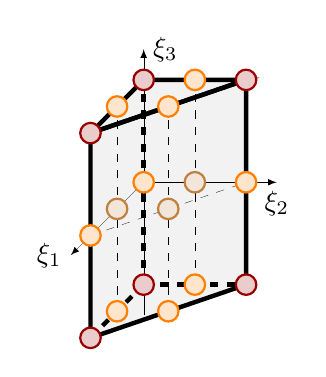
\begin{tikzpicture}[scale=1.3]
        \def\a{1}
        \def\b{1.35}
        \coordinate (x1) at (0,-\a,0);
        \coordinate (x2) at (0,-\a,\b);
        \coordinate (x3) at (\a,-\a,0);
        \coordinate (x4) at (0, \a,0);
        \coordinate (x5) at (0, \a,\b);
        \coordinate (x6) at (\a,\a,0);
        \coordinate (x7) at (0,-\a,\b/2);
        \coordinate (x8) at (\a/2,-\a,\b/2);
        \coordinate (x9) at (\a/2,-\a,0);
        \coordinate (x10) at (0,\a,\b/2);
        \coordinate (x11) at (\a/2,\a,\b/2);
        \coordinate (x12) at (\a/2,\a,0);
        \coordinate (x13) at (0,0,0);
        \coordinate (x14) at (0,0,\b);
        \coordinate (x15) at (\a,0,0);
        \coordinate (x16) at (0,0,\b/2);
        \coordinate (x17) at (\a/2,0,\b/2);
        \coordinate (x18) at (\a/2,0,0);
        %Shade
        \filldraw[gray!10] (x2) -- (x3) -- (x6) -- (x4) -- (x5) -- (x2);
        %Axis
        \draw[-latex,ultra thin] (0,0,0) -- (\a+0.3,0,0) node[below]{$\xi_2$};
        \draw[-latex,ultra thin] (0,-\a-0.3,0) -- (0,\a+0.3,0) node[right]{$\xi_3$};
        \draw[-latex,ultra thin] (0,0,0) -- (0,0,\b+0.5) node[left]{$\xi_1$};
        %Draw edges
        \draw[ultra thick,dashed] (x1) -- (x4);
        \draw[ultra thick,dashed] (x1) -- (x2);
        \draw[ultra thick,dashed] (x1) -- (x3);
        \draw[ultra thick] (x5) -- (x4) -- (x6) -- cycle;
        \draw[ultra thick] (x6) -- (x3) -- (x2) -- (x5) -- cycle;
        \draw[ultra thin,dashed] (x7) -- (x10);
        \draw[ultra thin,dashed] (x9) -- (x12);
        \draw[ultra thin,dashed] (x8) -- (x11);
        \draw[ultra thin,dashed] (x14) -- (x15);

        %Draw nodes
        \draw[fill=darkred!20, thick,draw=darkred] (x1) circle(0.1cm);
        \draw[fill=darkred!20, thick,draw=darkred] (x2) circle(0.1cm);
        \draw[fill=darkred!20, thick,draw=darkred] (x3) circle(0.1cm);
        \draw[fill=darkred!20, thick,draw=darkred] (x4) circle(0.1cm);
        \draw[fill=darkred!20, thick,draw=darkred] (x5) circle(0.1cm);
        \draw[fill=darkred!20, thick,draw=darkred] (x6) circle(0.1cm);
        \draw[fill=orange!20, thick,draw=orange] (x7) circle(0.1cm);
        \draw[fill=orange!20, thick,draw=orange] (x8) circle(0.1cm);
        \draw[fill=orange!20, thick,draw=orange] (x9) circle(0.1cm);
        \draw[fill=orange!20, thick,draw=orange] (x10) circle(0.1cm);
        \draw[fill=orange!20, thick,draw=orange] (x11) circle(0.1cm);
        \draw[fill=orange!20, thick,draw=orange] (x12) circle(0.1cm);
        \draw[fill=orange!20, thick,draw=orange] (x13) circle(0.1cm);
        \draw[fill=orange!20, thick,draw=orange] (x14) circle(0.1cm);
        \draw[fill=orange!20, thick,draw=orange] (x15) circle(0.1cm);
        \draw[fill=brown!20, thick,draw=brown] (x16) circle(0.1cm);
        \draw[fill=brown!20, thick,draw=brown] (x17) circle(0.1cm);
        \draw[fill=brown!20, thick,draw=brown] (x18) circle(0.1cm);
      \end{tikzpicture}
    \end{column}
    \begin{column}{0.33\textwidth}
      \centering
      \textbf{Triquadratic serendipity}
      \vspace{0.4cm}

      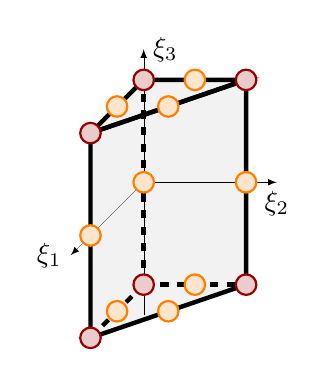
\begin{tikzpicture}[scale=1.3]
        \def\a{1}
        \def\b{1.35}
        \coordinate (x1) at (0,-\a,0);
        \coordinate (x2) at (0,-\a,\b);
        \coordinate (x3) at (\a,-\a,0);
        \coordinate (x4) at (0, \a,0);
        \coordinate (x5) at (0, \a,\b);
        \coordinate (x6) at (\a,\a,0);
        \coordinate (x7) at (0,-\a,\b/2);
        \coordinate (x8) at (\a/2,-\a,\b/2);
        \coordinate (x9) at (\a/2,-\a,0);
        \coordinate (x10) at (0,\a,\b/2);
        \coordinate (x11) at (\a/2,\a,\b/2);
        \coordinate (x12) at (\a/2,\a,0);
        \coordinate (x13) at (0,0,0);
        \coordinate (x14) at (0,0,\b);
        \coordinate (x15) at (\a,0,0);
        %Shade
        \filldraw[gray!10] (x2) -- (x3) -- (x6) -- (x4) -- (x5) -- (x2);
        %Axis
        \draw[-latex,ultra thin] (0,0,0) -- (\a+0.3,0,0) node[below]{$\xi_2$};
        \draw[-latex,ultra thin] (0,-\a-0.3,0) -- (0,\a+0.3,0) node[right]{$\xi_3$};
        \draw[-latex,ultra thin] (0,0,0) -- (0,0,\b+0.5) node[left]{$\xi_1$};
        %Draw edges
        \draw[ultra thick,dashed] (x1) -- (x4);
        \draw[ultra thick,dashed] (x1) -- (x2);
        \draw[ultra thick,dashed] (x1) -- (x3);
        \draw[ultra thick] (x5) -- (x4) -- (x6) -- cycle;
        \draw[ultra thick] (x6) -- (x3) -- (x2) -- (x5) -- cycle;
        %Draw nodes
        \draw[fill=darkred!20, thick,draw=darkred] (x1) circle(0.1cm);
        \draw[fill=darkred!20, thick,draw=darkred] (x2) circle(0.1cm);
        \draw[fill=darkred!20, thick,draw=darkred] (x3) circle(0.1cm);
        \draw[fill=darkred!20, thick,draw=darkred] (x4) circle(0.1cm);
        \draw[fill=darkred!20, thick,draw=darkred] (x5) circle(0.1cm);
        \draw[fill=darkred!20, thick,draw=darkred] (x6) circle(0.1cm);
        \draw[fill=orange!20, thick,draw=orange] (x7) circle(0.1cm);
        \draw[fill=orange!20, thick,draw=orange] (x8) circle(0.1cm);
        \draw[fill=orange!20, thick,draw=orange] (x9) circle(0.1cm);
        \draw[fill=orange!20, thick,draw=orange] (x10) circle(0.1cm);
        \draw[fill=orange!20, thick,draw=orange] (x11) circle(0.1cm);
        \draw[fill=orange!20, thick,draw=orange] (x12) circle(0.1cm);
        \draw[fill=orange!20, thick,draw=orange] (x13) circle(0.1cm);
        \draw[fill=orange!20, thick,draw=orange] (x14) circle(0.1cm);
        \draw[fill=orange!20, thick,draw=orange] (x15) circle(0.1cm);
      \end{tikzpicture}
    \end{column}
  \end{columns}
\end{frame}



\begin{frame}{Gauss-Legendre quadrature}
  \begin{itemize}
    \item Numerical integration helps automate the calculation of the elementary quantities ${}^e\mathbf K $, ${}^e\mathbf M$ and ${}^e\mathbf r$.
    \item Integration is approximated as:
          \begin{equation*}
            \int_{\Omega^a}f(\boldxi) d\boldxi \approx \sum_{i=1}^{r_1} \sum_{j=1}^{r_2} \sum_{k=1}^{r_3} \omega_i^1 \omega_j^2 \omega_k^3 f(\xi_1^i, \xi_2^j, \xi_3^k)
          \end{equation*}
          where $\xi_j^i$ are known as \emph{Gauss points} and $\omega_i^j$ are their associated \emph{Gauss weights}.
  \end{itemize}
  \begin{tcolorbox}[colback=darkred!10,colframe=darkred!40!black,]
    \begin{itemize}
      \item[\HandRight]  If $f$ is a polynomial of degree $d_i=2r_i-1$ in the variable $\xi_i$, then the Gauss-Legendre approximation formula is \textbf{exact}.
    \end{itemize}
  \end{tcolorbox}
\end{frame}

\begin{frame}{An illustration of Gauss points - 3d elements}
  \centering
  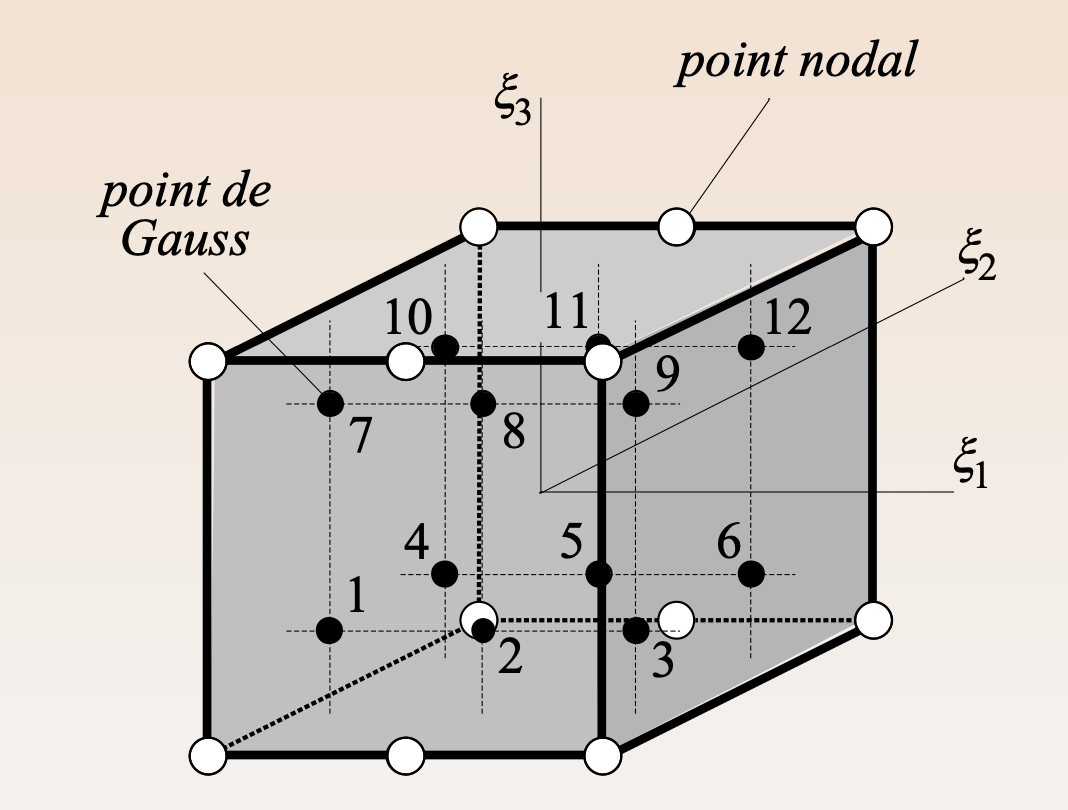
\includegraphics[height=5cm]{../images/gaussPoint1.png}\hspace{1cm}
  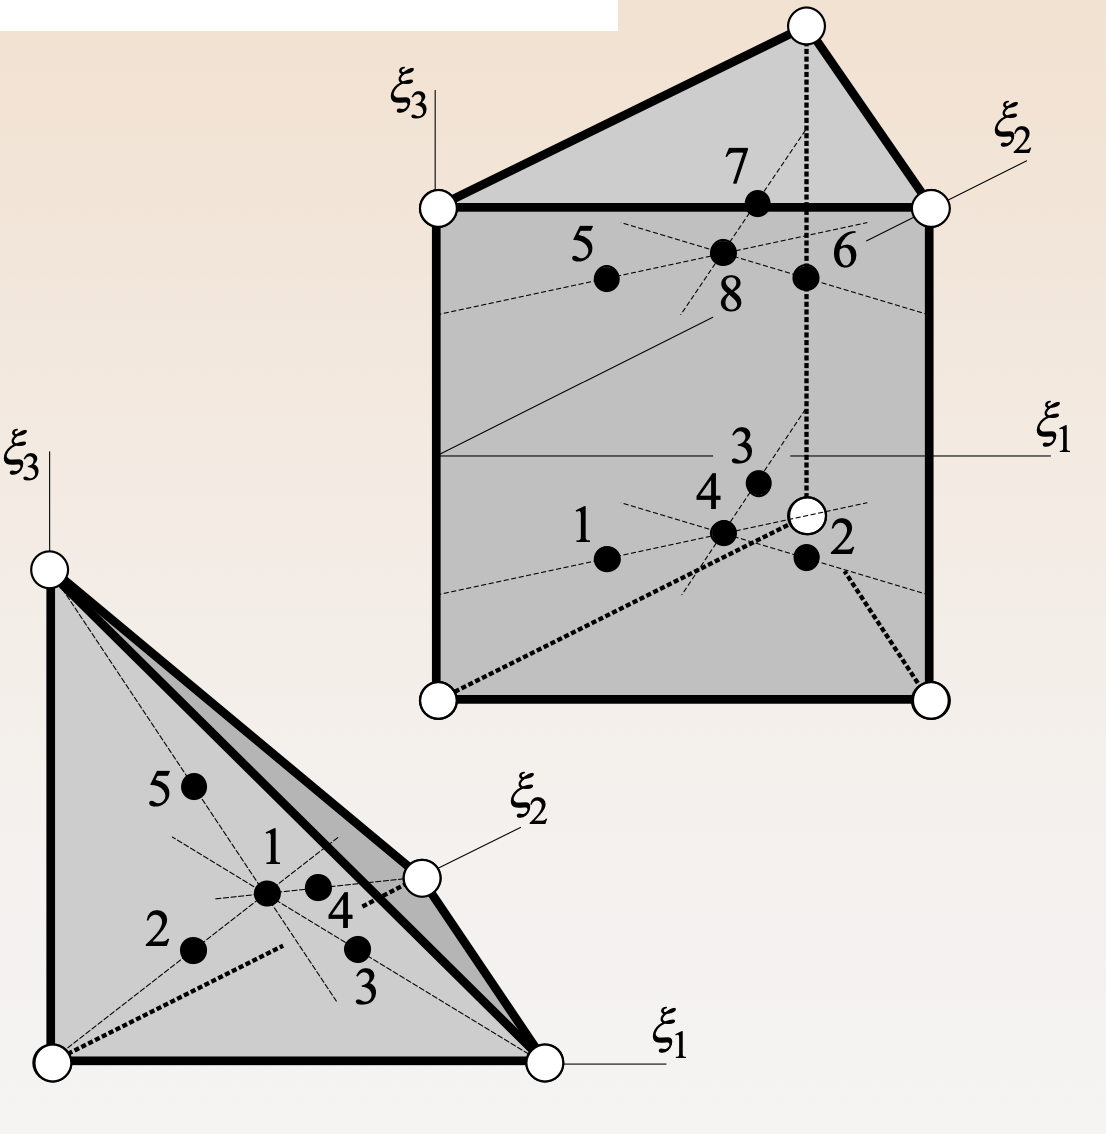
\includegraphics[height=5cm]{../images/gaussPoint2.png}
  \newline
  {\footnotesize (Credit: Thomas Gmür - Dynamique numérique des solides et des structures)}
\end{frame}


\begin{frame}{Number of Gauss points for exact integration}
  \begin{columns}
    \begin{column}{0.7\textwidth}
      \textbf{Trilinear hexahedral element}
      \begin{itemize}
        \item Basis functions are linear in each variable.
        \item Exact integration with:
              \begin{itemize}
                \item $2\times2\times2$ Gauss points for ${}^e\mathbf M$
                \item $1\times1\times1$ Gauss points for ${}^e\mathbf K$
              \end{itemize}
              if the element is not distorted.
        \item Note that in case of distortion:
              \begin{itemize}
                \item Jacobian is a function of $\boldxi$ : ${}^ej={}^ej(\boldxi)$\vspace{0.2cm}
                \item ${}^e\mathbf J^{-1}={}^e\mathbf J^{-1}(\boldxi)$ function of $\boldxi$ at the denominator.
                \item $\frac{\partial {}^e\mathbf H}{\partial \bold x}=\frac{\partial {}^a\mathbf H}{\partial \bold \xi} {}^e\mathbf J^{-1}$ is not a polynomial function of $\boldxi$ anymore.
              \end{itemize}
      \end{itemize}
    \end{column}
    % Right Column
    \begin{column}{0.3\textwidth}
      \centering
      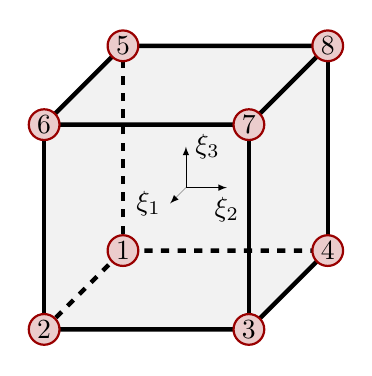
\begin{tikzpicture}[scale=1.3]
        \def\a{1}
        \coordinate (x1) at (-\a, -\a,-\a);
        \coordinate (x4) at (\a, -\a,-\a);
        \coordinate (x8) at (\a, \a,-\a);
        \coordinate (x5) at (-\a, \a,-\a);
        \coordinate (x2) at (-\a, -\a,\a);
        \coordinate (x3) at (\a, -\a,\a);
        \coordinate (x7) at (\a, \a,\a);
        \coordinate (x6) at (-\a, \a,\a);
        %Shade
        \filldraw[gray!10] (x1) -- (x2) -- (x3) -- (x4) -- cycle;
        \filldraw[gray!10] (x2) -- (x3) -- (x7) -- (x6) -- cycle;
        \filldraw[gray!10] (x3) -- (x4) -- (x8) -- (x7) -- cycle;
        \filldraw[gray!10] (x6) -- (x7) -- (x8) -- (x5) -- cycle;
        %Axis
        %Axis
        \draw[-latex,ultra thin] (0,0,0) -- (0.4,0,0) node[below]{$\xi_2$};
        \draw[-latex,ultra thin] (0,0,0) -- (0,0.4,0) node[right]{$\xi_3$};
        \draw[-latex,ultra thin] (0,0,0) -- (0,0,0.4) node[left]{$\xi_1$};
        %Draw edges
        \draw[ultra thick] (x6) -- (x7) -- (x8) -- (x5) -- cycle;
        \draw[ultra thick] (x2) -- (x3) -- (x4);
        \draw[ultra thick,dashed] (x2) -- (x1) -- (x4);
        \draw[ultra thick] (x2) -- (x6);
        \draw[ultra thick] (x3) -- (x7);
        \draw[ultra thick] (x4) -- (x8);
        \draw[ultra thick,dashed] (x1) -- (x5);
        %Draw nodes
        \draw[fill=darkred!20, thick,draw=darkred] (x1) node{1} circle(0.15cm);
        \draw[fill=darkred!20, thick,draw=darkred] (x2) node{2} circle(0.15cm);
        \draw[fill=darkred!20, thick,draw=darkred] (x3) node{3} circle(0.15cm);
        \draw[fill=darkred!20, thick,draw=darkred] (x4) node{4} circle(0.15cm);
        \draw[fill=darkred!20, thick,draw=darkred] (x5) node{5} circle(0.15cm);
        \draw[fill=darkred!20, thick,draw=darkred] (x6) node{6} circle(0.15cm);
        \draw[fill=darkred!20, thick,draw=darkred] (x7) node{7} circle(0.15cm);
        \draw[fill=darkred!20, thick,draw=darkred] (x8) node{8} circle(0.15cm);
      \end{tikzpicture}
    \end{column}
  \end{columns}
  \begin{tcolorbox}[colback=darkred!10,colframe=darkred!40!black,]
    \begin{itemize}
      \item[\HandRight] Gauss quadrature will never be exact in case of distortion.
    \end{itemize}
  \end{tcolorbox}
\end{frame}

\section{Types of structural analysis}

\begin{frame}{Static, modal, and transient analysis}
  \begin{itemize}
    \item \textbf{Static analysis}: determines deformations $\mathbf q$ due to constant loads.
          $$\mathbf K\mathbf q=\mathbf r$$
    \item  \textbf{Modal analysis}: studies dynamic properties in the frequency domain.
          $$\mathbf M\ddot{\mathbf q}(t)+\mathbf K\mathbf q(t)=\mathbf 0$$
          Natural frequency: key structural property  essential in structural design.
          \begin{itemize}
            \item Lower frequencies $\rightarrow$ higher displacement amplitudes $\rightarrow$ more dangerous.
            \item Resonance when external excitation frequency matches a natural frequency.
            \item Prolonged resonance $\rightarrow$ catastrophic failure.
          \end{itemize}
    \item   \textbf{Transient analysis}: examines time-dependent structural responses $\mathbf q(t)$  to time-dependent excitations $\mathbf r(t)$.
          $$\mathbf M\ddot{\mathbf q}(t)+\mathbf K\mathbf q(t)=\mathbf r(t)$$
  \end{itemize}
\end{frame}

\begin{frame}{Modal analysis overview}
  \vspace{-0.2cm}
  \begin{columns}
    \begin{column}{0.42\textwidth}
      \vspace{-0.3cm}
      \begin{center}
        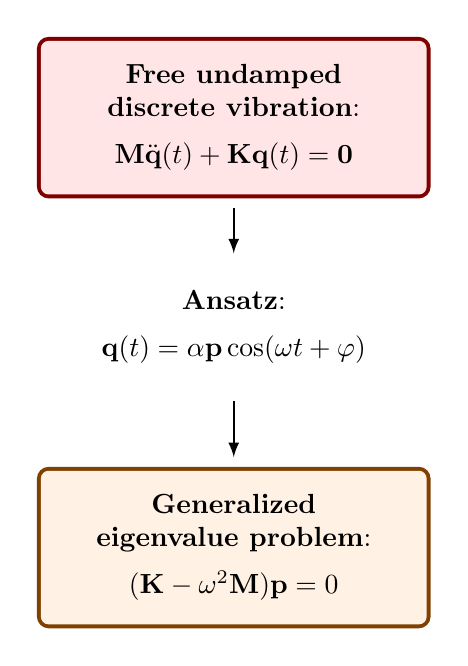
\begin{tikzpicture}[scale=0.7]
          \node (dvp) at (0,6) {
            \begin{tcolorbox}[colframe=red!50!black, colback=red!10, coltitle=black, rounded corners,width=5cm]
              \centering \textbf{Free undamped discrete vibration}: \\[5pt] $\mathbf{M} \ddot{\mathbf{q}}(t) + \mathbf{K} \mathbf{q}(t) = \mathbf{0}$
            \end{tcolorbox}
          };
          \node (ans) at (0,2.2) {
            \begin{tcolorbox}[colframe=white, colback=white, coltitle=black, rounded corners, width=5cm]
              \centering \textbf{Ansatz}: \\[5pt] $\mathbf q(t)=\alpha \mathbf p \cos(\omega t+\varphi)$
            \end{tcolorbox}
          };
          \node (gep) at (0,-1.8) {
            \begin{tcolorbox}[colframe=orange!50!black, colback=orange!10, coltitle=black, rounded corners,width=5cm]
              \centering \textbf{Generalized eigenvalue problem}: \\[5pt] $(\mathbf{K} - \omega^2 \mathbf{M}) \mathbf{p} = 0$
            \end{tcolorbox}
          };
          % Drawing arrows
          \draw[-latex, thick] (dvp.south) -- (ans.north);
          \draw[-latex, thick] (ans.south) -- (gep.north);
        \end{tikzpicture}
      \end{center}
    \end{column}
    \begin{column}{0.54\textwidth}
      \textbf{Solving the eigenvalue problem:}
      $$n=\text{dim}(\mathbf K)=\text{dim}(\mathbf M)$$
      \begin{block}{}
        \textbf{Eigenvalues} (\emph{natural frequencies} squared): $\lambda_j=\omega_j^2$ are the roots of the characteristic polynomial:
        $$\text{det}(\mathbf K-\lambda\mathbf M)=0.$$
      \end{block}
      \begin{block}{}
        \textbf{Eigenvectors} (\emph{modal shapes}): $\mathbf p_j$ are the solution of the equation
        $$(\mathbf{K} - \lambda_j \mathbf{M})\mathbf p_j=\mathbf 0.$$
      \end{block}
    \end{column}
  \end{columns}
\end{frame}


\begin{frame}{A priori error estimates for eigenvalues and eigenvectors}
  \begin{tcolorbox}[colback=darkred!10,colframe=darkred!40!black]
    \vspace{-0.5cm}
    \begin{align*}
      \lambda_i^e \leq \lambda_i                    & \leq \lambda_i^e + c\, h^{2(m-k+1)}\, ({\lambda_i^e})^{m+1}  \\
      \| \boldsymbol{p}_i - \boldsymbol{p}_i^e \|_0 & \leq c\, h^{\min(m+1, 2(m-k+1))}\, ({\lambda_i^e})^{(m+1)/2}
    \end{align*}
  \end{tcolorbox}
  \begin{itemize}
    \setlength\itemsep{0.5em}
    \item \( \lambda_i \) are the \emph{approximated} eigenvalues and \(\boldsymbol p_i \) the corresponding eigenvectors,
    \item  \( \lambda_i^e\) are the \emph{exact} eigenvalues and \(\boldsymbol p_i^e \) the corresponding exact eigenvectors,
    \item \( h \) represents the characteristic mesh size,
    \item \( m \) is the degree of the highest complete polynomial used,
    \item \( k \) is the the highest derivative order appearing in the weak form,
    \item \( c \) is a constant independent of \( h \),
    \item  \( \| \cdot \|_0 \) Euclidean \( L^2 \) norm.
  \end{itemize}
\end{frame}

\begin{frame}{Rigid body modes}
  In the semi-discrete weak form obtained via finite element discretization:
  \begin{itemize}
    \item The \textbf{mass matrix} \( \mathbf{M} \) is symmetric and strictly positive definite.
    \item The \textbf{stiffness matrix} \( \mathbf{K} \) is symmetric and positive semi-definite:
          \[
            \mathbf{K} \mathbf{p} = \mathbf{0} \quad \text{for certain nonzero vectors } \mathbf{p}.
          \]
  \end{itemize}
  Consequently, the eigenvalues \( \lambda_j\) of the generalized eigenvalue problem are all real and non-negative:
  \[
    0 \,\leq\, \omega_1 \leq \omega_2 \leq \dots \leq \omega_n.
  \]

  \begin{block}{}
    \textbf{Rigid body modes:} zero eigenvalues (i.e., \( \omega_j = 0 \)) correspond to \emph{rigid body motions}, where the system undergoes displacement without internal deformation.
  \end{block}
\end{frame}

\begin{frame}{Orthonormalization of mode shapes}
  \begin{block}{}
    Let $\mathbf p_i$ and $\mathbf p_j$ two eigenvectors corresponding to the  eigenvalues $\lambda_i$ and $\lambda_j$, then
    $$
      \mathbf p_i^T\mathbf M\mathbf p_j  =\delta_{ij}
      \qquad\text{and}\qquad
      \mathbf p_i^T\mathbf K\mathbf p_j  =\omega_i^2\delta_{ij}
    $$
    where $\delta_{ij}$ represent Kronecker symbol.
  \end{block}
  \textbf{Consequences:} if we organize the modal vectors $\mathbf p_i$ in a so-called modal matrix $\mathbf P$:
  $$\mathbf P=\left[ \begin{array}{c;{2pt/2pt}c;{2pt/2pt}c;{2pt/2pt}c}
        \mathbf p_{1} & \mathbf p_{2} & \dots & \mathbf p_{n} \\
      \end{array}\right]$$
  then
  \begin{block}{}
    $$  \mathbf P^T\mathbf M\mathbf P  =\mathbf I       \qquad\text{and}\qquad
      \mathbf P^T\mathbf K\mathbf P  =\mathbf\Lambda$$
    where $\mathbf I$ is the identity matrix of order $n$ and $\mathbf\Lambda$ the \emph{spectral matrix}:
    $$\mathbf\Lambda=\text{diag}(\lambda_1,\dots,\lambda_n)=\text{diag}(\omega_1^2,\dots,\omega_n^2).$$
  \end{block}
\end{frame}

\begin{frame}{Small and large scale problems}
  \vspace{-0.3cm}
  \begin{tcolorbox}[colback=darkred!10,colframe=darkred!40!black]
    Economical computation algorithms for extracting $(\lambda_j,\mathbf p_j)$ for $1\leq j \leq n_{modes}$ are required in practical applications, where $n_{modes}\ll n$ is the number of desired eigenpairs.
  \end{tcolorbox}

  \begin{columns}[T]
    \begin{column}{.48\textwidth}
      \textbf{Small-scale problems}
      \begin{itemize}
        \item system matrices are of modest size $n\leq 250$ or $250\leq n \leq 2500$ and small bandwidth matrices.
        \item An explicit reduction to standard eigenvalue form is typically employed:
              \begin{itemize}
                \item\emph{Generalized Jacobi method}
                \item \emph{Householder QR-algorithm}
              \end{itemize}
      \end{itemize}
    \end{column}
    \begin{column}{.48\textwidth}
      \textbf{Large-scale problems}
      \begin{itemize}
        \item $n\geq 2500$.
        \item The most effective algorithms are:
              \begin{itemize}
                \item \emph{Subspace iteration method},
                \item \emph{Lanczos' method},
                \item \emph{Irons-Guyan reduction method},
                \item \emph{Arnoldi method}
                \item \emph{Davidson method}.
              \end{itemize}
      \end{itemize}
    \end{column}
  \end{columns}
\end{frame}

\begin{frame}{Rayleigh's quotient}
  \small
  \begin{itemize}
    \item Rayleigh's quotient of a generic vector $\mathbf w$:
          \[
            \mathcal R(\mathbf w) = \frac{\mathbf w^T \mathbf K \mathbf w}{\mathbf w^T \mathbf M \mathbf w}
          \]
    \item For a given eigenvector \( \mathbf{p}_i  \), the Rayleigh quotient provides the corresponding eigenvalue \( \omega_i^2 \):$$\mathcal R(\mathbf p_i) = \lambda_i= \omega_i^2.$$
    \item The first variation of Rayleigh's quotient is zero at the eigenvectors:
          \[
            \delta \mathcal{R}(\mathbf{w}) = 0 \quad \text{if and only if} \quad \mathbf{w} = \mathbf{p}_i,
          \]
          where \(\mathbf{p}_i\) is an eigenvector.
    \item \textbf{Bounding theorem:}
          \vspace{0.2cm}
          \(
          \lambda_1 \leq \mathcal{R}(\mathbf{w}) \leq \lambda_n
          \)
  \end{itemize}
  \begin{tcolorbox}[colback=darkred!10,colframe=darkred!40!black]
    The Rayleigh quotient can be used to approximate the smallest eigenvalue \( \lambda_1 = \omega_1^2 \) by minimizing \( \mathcal R(\mathbf w) \) over all non-zero vectors \( \mathbf w \).
  \end{tcolorbox}
\end{frame}


\begin{frame}{General idea of inverse and forward iteration}
  \vspace{-0.2cm}
  \small
  \begin{block}{}
    \textbf{Goal:} compute \textbf{one} eigenvector of the generalized eigenproblem \( \mathbf K\mathbf p = \lambda\mathbf M \mathbf p \).
  \end{block}
  \textbf{Idea:} Use an \emph{iterative} improvement of an assumed eigenvector.
  \begin{itemize}
    \item Start from an arbitrary vector $\mathbf p^{(0)}$.
    \item Generate a sequence of vectors $\mathbf p^{(1)}, \mathbf p^{(2)}, \dots$ that converge to an eigenvector.
    \item  Compute an approximate eigenvalue using Rayleigh's quotient:
          \[
            \lambda^{(k)} = \mathcal R(\mathbf p^{(k)}).
          \]
  \end{itemize}
  \begin{columns}[T]
    \begin{column}{0.5\textwidth}
      \textbf{Inverse iteration:}
      \begin{itemize}
        \item Form a \emph{“force”} vector:
              \(
              \mathbf R_1 = \mathbf M \mathbf p^{(0)}.
              \)
        \item Solve the static-like equilibrium problem:
              \[
                \mathbf K \mathbf p^{(1)} = \mathbf R_1,
              \]
        \item Repeat until convergence is met.
      \end{itemize}
    \end{column}
    \begin{column}{0.5\textwidth}
      \textbf{Forward iteration:}
      \begin{itemize}
        \item Compute $\mathbf R_1 = \mathbf K \mathbf p^{(0)}$.
        \item Solve
              \[
                \mathbf M \mathbf p^{(1)} = \mathbf R_1 ,
              \]
        \item Repeat until convergence is met.
      \end{itemize}
    \end{column}
  \end{columns}
\end{frame}


\begin{frame}{Inverse iteration algorithm}
  \small
  \textbf{Goal:} Compute \textbf{one} eigenvector using iterative refinement. \\[2mm]

  \textbf{Algorithm:}
  \begin{enumerate}
    \item Choose initial guess \(\mathbf p^{(0)}\), spectral shift \(\sigma\), tolerance \(\varepsilon\).
    \item Define shifted stiffness: \(\mathbf K_\sigma = \mathbf K + \sigma \mathbf M\)
    \item For \(k = 1,2,\dots\) until convergence:
          \begin{enumerate}
            \item Solve: \(\mathbf K_\sigma \, \bar{\mathbf p}^{(k)} = \mathbf M \, \mathbf p^{(k-1)}\)
            \item Normalize: \(\mathbf p^{(k)} = \bar{\mathbf p}^{(k)} / \sqrt{(\bar{\mathbf p}^{(k)})^T \mathbf M \bar{\mathbf p}^{(k)}}\)
            \item Check: \(\|\mathbf p^{(k)} - \mathbf p^{(k-1)}\| < \varepsilon\)
          \end{enumerate}
    \item Output: eigenvector \(\mathbf p^{(k)}\), eigenvalue \(\lambda^{(k)} = \mathcal R(\mathbf p^{(k)})\)
  \end{enumerate}

  \vspace{2mm}
  \textbf{Key points:}
  \begin{itemize}
    \item Converges to eigenvector closest to \(\sigma\) if \(\mathbf p^{(0)}\) not \(\mathbf M\)-orthogonal to it.
    \item Without shift (\(\sigma=0\)) $\to$ eigenvector of smallest eigenvalue.
    \item Convergence rate: \(\rho = \frac{|\lambda_j - \sigma|}{|\lambda_{j+1}-\sigma|}\)
  \end{itemize}
\end{frame}

\begin{frame}{Inverse iteration on \( q \) vectors}
  Suppose that we perform a simultaneous inverse iteration on \( q \) eigenvectors:
  \[
    \mathbf P^{(k)} = (\mathbf K^{-1}\mathbf M)\mathbf P^{(k-1)}=\dots = (\mathbf K^{-1}\mathbf M)^k\, \mathbf P^{(0)}
  \]
  \vspace{-0.5cm}
  \begin{block}{}
    Define the subspace \( \mathcal S^{(k)} \) of rank \( q \), spanned by the vectors \( \{\mathbf p_i^{(k)}\} \).  $\mathbf  P^{(k)}=[\mathbf p^{(k)}_1,\dots,\mathbf p^{(k)}_q]$ forms a \emph{non-orthogonal} basis of vector spaces \( \mathcal S^{(k)} \).
  \end{block}
  \begin{itemize}
    \item[\XSolidBrush] All columns of \(\mathbf  P^{(k)} \) tend toward \( \mathbf  p_1 \)
    \item[\XSolidBrush]  Collinearity if no orthogonalization is applied !
  \end{itemize}

  \begin{tcolorbox}[colback=darkred!10,colframe=darkred!40!black]
    \begin{center}
      \textbf{Orthogonalization} of vectors \(\mathbf p_i^{(k)} \) at each iteration needed !
    \end{center}
  \end{tcolorbox}
\end{frame}

\begin{frame}{Subspace iteration method}
  \small
  \textbf{Goal:} Compute the lowest \(n_{modes} \ll n\) eigenpairs \((\mathbf p_i, \lambda_i)\) of using a \(q\)-dimensional subspace iteration.\\[1mm]

  \textbf{Key ideas and advantages:}
  \begin{itemize}
    \item Iteration is performed on a subspace \(\mathcal S_k = \text{span}(\mathbf p_1^{(k)},\dots,\mathbf p_q^{(k)})\), not individual vectors.
    \item At each iteration, inverse iteration is applied to all \(q\) vectors in the subspace and then orthogonalized via Rayleigh-Ritz.
    \item Easier to initialize a subspace close to the span of required eigenvectors than individual vectors.
  \end{itemize}
  \begin{center}
    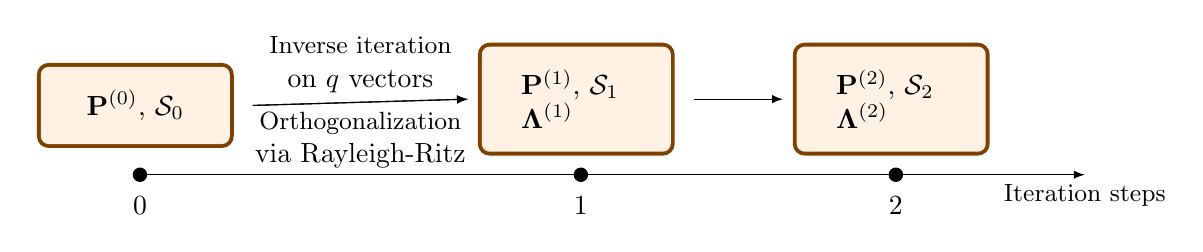
\begin{tikzpicture}[scale=0.8]
      \draw[-latex] (0,0) -- (15,0) node[below] {\small Iteration steps};
      \filldraw (0,0) circle (3pt); % Marker
      \filldraw (7,0) circle (3pt); % Marker
      \filldraw (12,0) circle (3pt); % Marker
      \node[align=center,below] at (0,-0.2) {$0$};
      \node[align=center, below] at (7,-0.2) {$1$};
      \node[align=center,below] at (12,-0.2) {$2$};
      % Drawing boxes
      \node[align=center] (iter0) at (0,1.1) {
        \begin{tcolorbox}[colframe=orange!50!black, colback=orange!10, coltitle=black, rounded corners,width=2.5cm]
          \centering $\mathbf P^{(0)}$, $\mathcal S_0$
        \end{tcolorbox}
      };

      \node[align=center] (iter1)at (7,1.2) {\begin{tcolorbox}[colframe=orange!50!black, colback=orange!10, coltitle=black, rounded corners,width=2.5cm]
          $\mathbf P^{(1)}$, $\mathcal S_{1}$ \\  $\mathbf \Lambda^{(1)}$
        \end{tcolorbox}
      };

      \node[align=center] (iter2) at (12,1.2) {\begin{tcolorbox}[colframe=orange!50!black, colback=orange!10, coltitle=black, rounded corners,width=2.5cm]
          $\mathbf P^{(2)}$, $\mathcal S_{2}$ \\  $\mathbf \Lambda^{(2)}$
        \end{tcolorbox}
      };

      % Drawing arrows
      \draw[-latex] (iter0.east) -- (iter1.west)  node[midway, above, align=center] {\small Inverse iteration \\ on $q$ vectors};
      \draw[-latex] (iter0.east) -- (iter1.west)  node[midway, below, align=center] {\small Orthogonalization \\ via Rayleigh-Ritz};
      \draw[-latex] (iter1.east) -- (iter2.west);
    \end{tikzpicture}
  \end{center}
\end{frame}

\begin{frame}{Subspace iteration algorithm}
  \small
  \textbf{Inputs:} \(\mathbf K, \mathbf M, n_{modes}, q>n_{modes}, \mathbf P^{(0)}\in \mathbb{R}^{n\times q}, \sigma, \varepsilon\)\\[1mm]

  \textbf{Iteration:} For \(k=1,2,\dots\) until convergence:
  \begin{enumerate}
    \item Solve \( \mathbf K_\sigma \, \overline{\mathbf P^{(k)}} = \mathbf M \mathbf P^{(k-1)} \) (inverse iteration on \(q\) vectors)
    \item Project and solve small eigenproblem:
          \[
            \mathbf K^{(k)} = (\overline{\mathbf P^{(k)}})^T \mathbf K \overline{\mathbf P^{(k)}}, \quad
            \mathbf M^{(k)} = (\overline{\mathbf P^{(k)}})^T \mathbf M \overline{\mathbf P^{(k)}}
          \]
          \[
            \mathbf K^{(k)} \mathbf Z^{(k)} = \mathbf M^{(k)} \mathbf Z^{(k)} \mathbf \Lambda^{(k)}
          \]
    \item Update modal matrix: \( \mathbf P^{(k)} = \overline{\mathbf P^{(k)}} \mathbf Z^{(k)} \), ensure \( (\mathbf P^{(k)})^T \mathbf M \mathbf P^{(k)} = \mathbf I \)
    \item Check convergence: \( \frac{|\lambda_i^{(k)} - \lambda_i^{(k-1)}|}{\lambda_i^{(k)}} < \varepsilon \)
  \end{enumerate}

  \textbf{Notes:}
  \begin{itemize}
    \item Orthogonalization is critical to prevent collinearity of iteration vectors.
    \item Starting vectors should be linearly independent; larger \(q\) increases convergence rate but also computational cost.
    \item After convergence, use Sturm sequence to verify the number of eigenvalues computed.
  \end{itemize}
\end{frame}


\begin{frame}{Starting iteration vectors $\mathbf P^{(0)}$}
  \begin{itemize}
    \item The starting iteration vectors in $\mathbf P^{(0)}$ should not be too close to each other, i.e., they should be linearly independent.
    \item Higher convergence rate can be obtained by increasing $q$. However, using more iteration vectors will also increase the computer effort for one iteration. In practice
          $$q=\min(2n_{modes},\, n_{modes} + 8)$$
  \end{itemize}
  \begin{tcolorbox}[colback=darkred!10,colframe=darkred!40!black]
    \textbf{Empirical guidelines}
    \begin{itemize}
      \item The first column of $\mathbf P^{(0)}$ should be the diagonal of $\mathbf M$. This ensures that all mass degrees of freedom are excited.
      \item The other columns in $\mathbf P^{(0)}$, except for the last column, should be unit vectors $\mathbf e_i$, with entries $+1$ at the degrees of freedom with the smallest ratios $k_{ii}/m_{ii}$, and the last column in $\mathbf P^{(0)}$ should be a random vector with values in $[0,1]$.
    \end{itemize}
  \end{tcolorbox}
\end{frame}

\begin{frame}{Convergence of the subspace iteration method}
  \begin{itemize}
    \item Iteration is performed with $q$ vectors, $q > n_{modes}$, but convergence is measured only on the approximations obtained for the $n_{modes}$ smallest eigenvalues.
    \item If the starting iteration vectors in $\mathbf P^{(0)}$, are not orthogonal to any one of the required eigenvectors $\mathbf p_1,\dots, \mathbf p_{n_{modes}}$, then as $k\to \infty$
          $$\tilde{\mathcal S}_k=\text{span}(\mathbf p^{(k)}_1, \dots, \mathbf p^{(k)}_{n_{modes}})\to \mathcal S_\infty = \text{span}(\mathbf p_1, \dots, \mathbf p_{n_{modes}})$$\
    \item  Assuming that in the iteration
          the vectors in $\mathbf P^{(k+1)}$ are ordered in such way that the $i$-th diagonal element in $\mathbf \Lambda^{(k+1)}$ is larger
          than the $(i - 1)$-st element for $i = 2,\dots, p$, then the $i$-th column in $\mathbf P^{(k+1)}$ converges to $\mathbf p_i$ and the convergence rate is
          $$\lambda_i/\lambda_{p+1}$$
          Although this is an asymptotic convergence rate, it indicates that the smallest eigenvalues converge fastest.
  \end{itemize}
\end{frame}

\begin{frame}{Final Sturm sequence check}
  \begin{block}{}
    After convergence is achieved, a final check based on the Sturm sequence property can be performed to ensure that the number of computed eigenvalues below a certain value is correct.
  \end{block}

  \begin{itemize}
    \item The Sturm sequence property states that the number of eigenvalues of the generalized eigenvalue problem \( \mathbf K\mathbf p = \lambda\mathbf M \mathbf p \) that are less than a given value \( \lambda^* \) is equal to the number of negative pivots obtained when performing an \( \mathbf L\mathbf  D\mathbf  L^T \) factorization of the matrix \( \mathbf K - \lambda^* \mathbf M \).
    \item This property can be used to verify that the number of computed eigenvalues below a certain threshold matches the expected count, providing an additional layer of validation for the results obtained from the subspace iteration method.
  \end{itemize}
\end{frame}

\end{document}





